\documentclass[mathserif]{beamer}
\usepackage{beamerthemeshadow}
\usepackage{beamerthemesplit}
%\usetheme{shadow}
\usecolortheme{default}
\setbeamertemplate{footline}[frame number]
\useinnertheme[shadow=true]{rounded}
%\setbeamertemplate{footline}{\insertframenumber/\inserttotalframenumber}
%\useoutertheme{infolines}
%\setbeamertemplate{headline}{} % removes the headline that infolines inserts

%\usetheme{boxes}
%\usepackage{amsmass}
%\usepackage{amssymb,amsfonts,url}


\usepackage{algorithm}
\usepackage{algorithmic}

\usepackage{graphicx}
\graphicspath{{Problems/}}

%\usepackage{CJK}
%\usepackage{pinyin}

%    \begin{figure}
%        \centering
%        \includegraphics[width=0.8\textwidth]{newGeneRep.eps}
%    \end{figure}

% \begin{figure}%
%   \begin{center}%
%     \begin{minipage}{0.70\textwidth}%
%      \includegraphics[width=1.0\textwidth]{comp25000.eps}%
%     \end{minipage}%
%     \begin{minipage}{0.30\textwidth}
%      \includegraphics[width=1.0\textwidth]{comparelabel.eps}%
%     \end{minipage}%
%   \end{center}
% \end{figure}

% \begin{table}
%   {\begin{tabular}{l|rrr}\hline
%       & \multicolumn{3}{c}{Actual number of DCJ operations}\\
%       \# genes &\# genes $\times 1$&\# genes $\times 2$&\# genes  $\times 3$ \\
% \hline
%      (a)~25,000 & 0.5\% ~~&  0.9\% ~~& 1.7\%~~\\
%       (b)~10,000 & 0.8\%~~ &  1.4\% ~~& 2.7\%~~\\
%      (c)~ 1,000 & 2.7\%~~ & 4.7\%~~ & 14.7\%~~\\ \hline
%     \end{tabular}} {}%
% \end{table}

% \begin{eqnarray}
% T(n) &=&  \sum_{i=1}^n C_i \\
%      &=&  \# PUSH + \#POP \\
%      &<& 2\times \#PUSH \\
%      &<& 2n \\
% \end{eqnarray}

% \[ 
% \begin{matrix}
% \begin{pmatrix}
% C_{11} & C_{12} \\ 
% C_{21} & C_{22} 
% \end{pmatrix}
% =
% \begin{pmatrix}
% A_{11} & A_{12} \\ 
% A_{21} & A_{22}  
% \end{pmatrix}
% 
% \begin{pmatrix}
% B_{11} & B_{12} \\ 
% B_{21} & B_{22}  
%  
% \end{pmatrix}
%     
%    \end{matrix}
% \]
% 
% 
% \begin{eqnarray}
%  C_{11} &=& (A_{11}\times B_{11}) + (A_{12} \times B_{21}) \\
% C_{12} &=& (A_{11}\times B_{12}) + (A_{12} \times B_{22}) \\
% C_{21} &=& (A_{21}\times B_{11}) + (A_{22} \times B_{21}) \\
% C_{22} &=& (A_{21}\times B_{12}) + (A_{22} \times B_{22}) 
% \end{eqnarray}
% \begin{figure}%
%      \begin{minipage}{0.32\textwidth}%
%       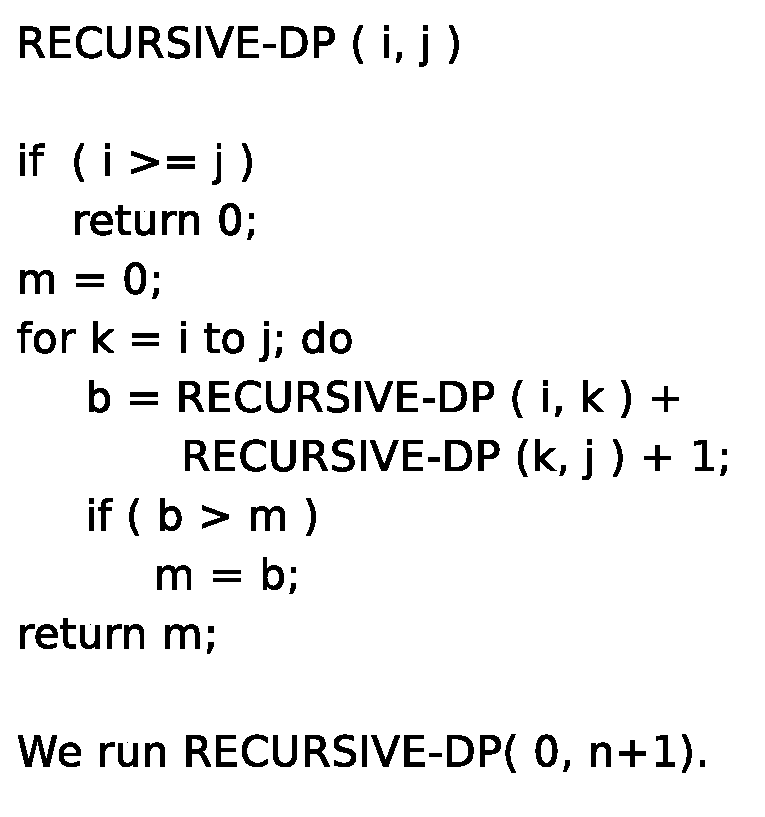
\includegraphics[width=1.0\textwidth]{L7-intervalschedulingdpalgo.eps}%
%      \end{minipage}%
%  \quad
%      \begin{minipage}{0.30\textwidth}
%       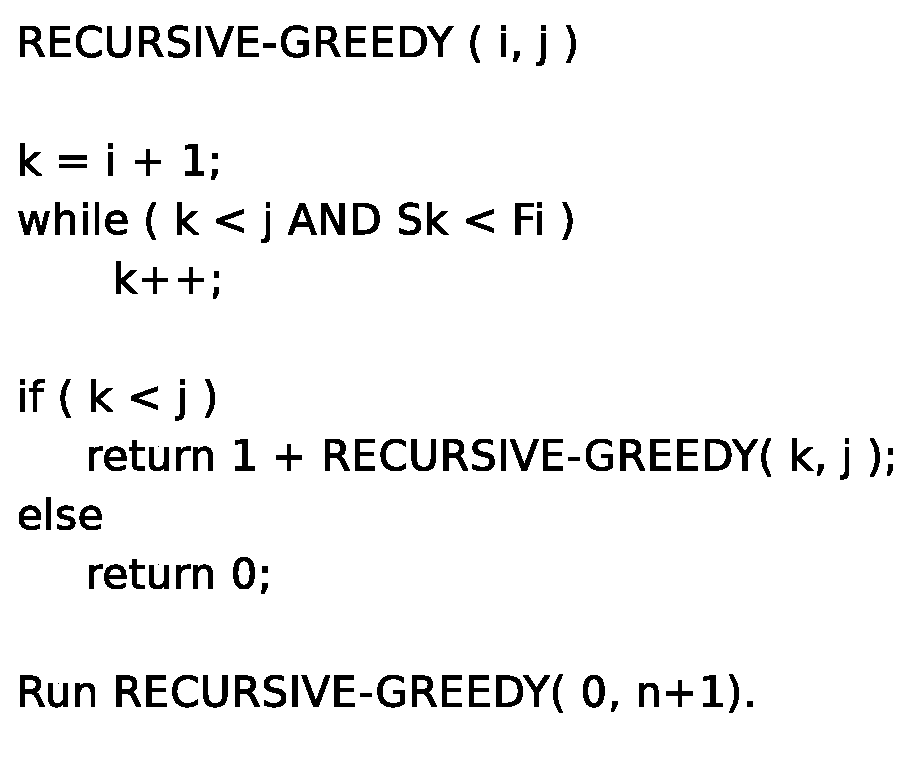
\includegraphics[width=1.0\textwidth]{L7-intervalschedulinggreedyalgo.eps}%
%      \end{minipage}%
%  \quad
%       \begin{minipage}{0.25\textwidth}
%       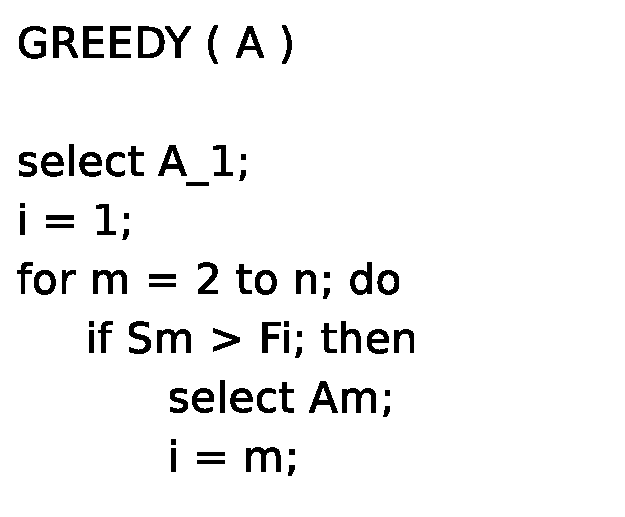
\includegraphics[width=1.0\textwidth]{L7-intervalschedulinggreedyalgo2.eps}%
%      \end{minipage}%
% 
%  \end{figure}

\title{CS711008Z  Algorithm Design and Analysis }
\subtitle{ Lecture 10. Algorithm design technique: Network flow and its applications
\footnote{The slides are made based on Chapter 7 of {\it Introduction to algorithms}, {\it Combinatorial optimization algorithm and complexity} by C. H. Papadimitriou and K. Steiglitz, the classical papers by Kuhn, Edmonds, etc. in the book {\it 50 Years of Integer Programming 1958-2008: From the Early Years to the State-of-the-Art.}  } }
\author{Dongbo Bu } 
\institute{ {\small Institute of Computing Technology \\ 
Chinese Academy of Sciences, Beijing, China}}

\date{}

\begin{document}
%\begin{CJK}{UTF8}{cyberbit}

\frame{\titlepage}

\frame{
\frametitle{Outline}
\begin{itemize}
\item Extensions of {\sc MaximumFlow} problem: undirected network; {\sc Circulation} with  multiple sources $\&$ multiple sinks;  {\sc Circulation}  with lower bound of capacity; {\sc Minimum Cost Flow}; 
\item Solving practical problems using network flow and primal\_dual techniques: 
  \begin{enumerate}
  \item Partitioning a set: {\sc ImageSegmentation}, {\sc ProjectSelection}, {\sc ProteinDomainParsing}; 
  \item Finding paths: {\sc FlightScheduling}, {\sc Disjoint Paths}, {\sc BaseballElimination};  
  \item Decomposing numbers: {\sc BaseballElimination};
\item Constructing matches: {\sc BipartiteMatching}, {\sc SurveyDesign};
  \end{enumerate}
\item Extensions of matching: \begin{small} {\sc BipartiteMatching}, {\sc WeightedBipartiteMatching}, {\sc GeneralGraphMatching}, {\sc WeightedGeneralGraphMatching}; \end{small}
\item A brief history of network flow.
\end{itemize}
}

\frame{
\begin{block}{}
 Extensions of {\sc MaximumFlow} problem
\end{block}
}

\frame{
\frametitle{Extensions }

Four extensions of {\sc MaximumFlow} problem: 
\begin{block}{}
 \begin{enumerate}
  \item {\sc MaximumFlow} for undirected network; \\
  \ \\
  \item {\sc Circulation} with multiple sources and multiple sinks; \\
  \ \\
  \item  {\sc Circulation}  with lower bound for capacity;  \\
  \ \\
  \item {\sc Minimum Cost Flow};
  \end{enumerate}
\end{block}
}

\frame{
\begin{block}{}
Extension 1: {\sc Maximum Flow} for undirected network
\end{block}
}

\frame{
\frametitle{ Extension 1: {\sc Maximum Flow} for undirected network}

\begin{block}{}
{\bf INPUT: } \\ an \textcolor{blue}{\bf undirected} network $G=<V, E>$, each edge $e$ has a capacity $C(e) > 0$. Two special nodes: \textcolor{red}{\bf source $s$} and \textcolor{red}{\bf sink $t$}; \\ 
{\bf OUTPUT: } \\ for each edge $e$, to assign a flow $f(e)$ to maximize the flow value $\sum_{e=(s,v)} f(e)$. 
\end{block}

Flow properties: 
\begin{enumerate}
 \item (Capacity restriction):  \textcolor{red}{$0 \leq f(u, v) + f(v, u) \leq C(u, v)$} for any $(u,v) \in E$;
  \item (Conservation restriction):  $f^{in} (v) = f^{out} (v)$ for any node $v\in V$ except for $s$ and $t$. 
\end{enumerate}
} 


\frame{
\frametitle{ Example }

\begin{figure}
 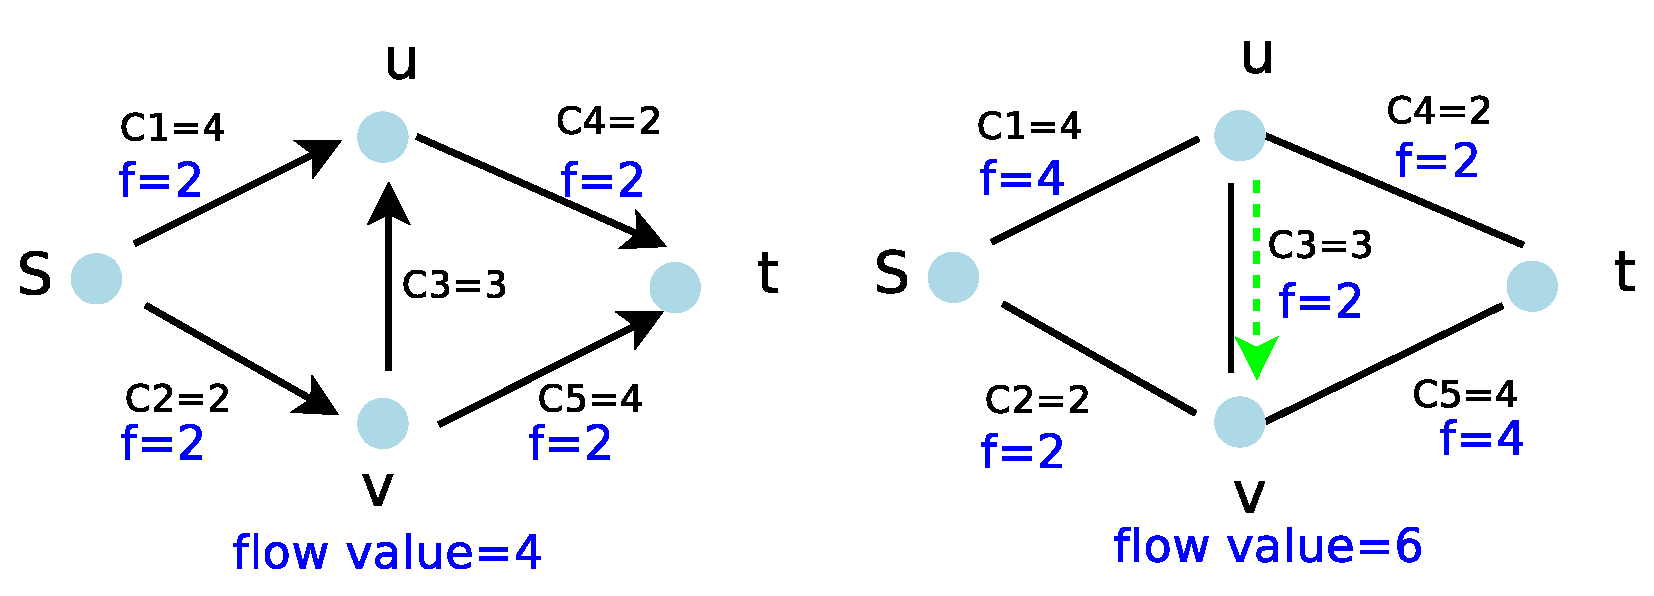
\includegraphics[width=3.3in] {L10-networkflowundirectedexample.eps}
\end{figure}

Note: On the directed network, the maximum flow value is $4$; in contrast, on the undirected network, the maximum flow value is $6$. 
}

\frame{
\frametitle{ Algorithm } 

Maximum-flow algorithm for undirected network $G$
  \begin{algorithmic}[1]
    \STATE Transforming the undirected network $G$ to a directed network $G'$; 
    \STATE Calculating the maximum flow for $G'$ by using Ford-Fulkerson algorithm;
    \STATE Revising the flow to meet the capacity restrictions; 
  \end{algorithmic}
}

\frame{
\frametitle{ Step 1: changing undirected network to directed network }

\begin{itemize}
 \item 
Transformation: an undirected network $G$ is transformed into a directed network $G'$ through: 
\begin{enumerate}
 \item adding edges:  for each edge $(u,v)$ of $G$, introducing two edges $e=(u,v)$ and $e'=(v,u)$ to $G'$; 
\item setting capcities: setting $C(e')=C(e)$. 
\end{enumerate}

\begin{figure}
 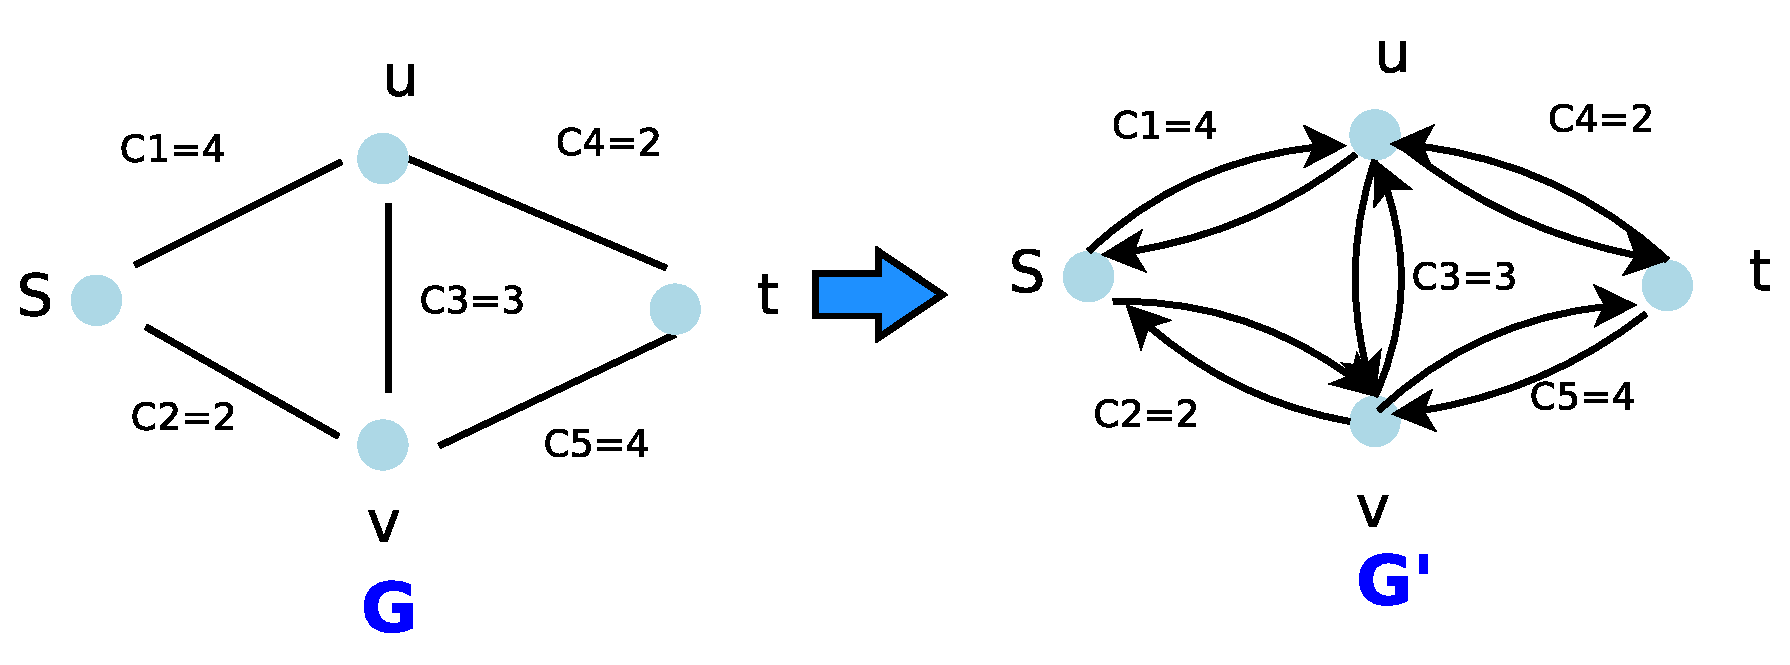
\includegraphics[width=3.6in] {L10-networkflowundirecteddirected.eps}
\end{figure}
\end{itemize}
}

\frame{
\frametitle{ Step 2: calculating the maximum flow for $G'$ }


\begin{figure}
 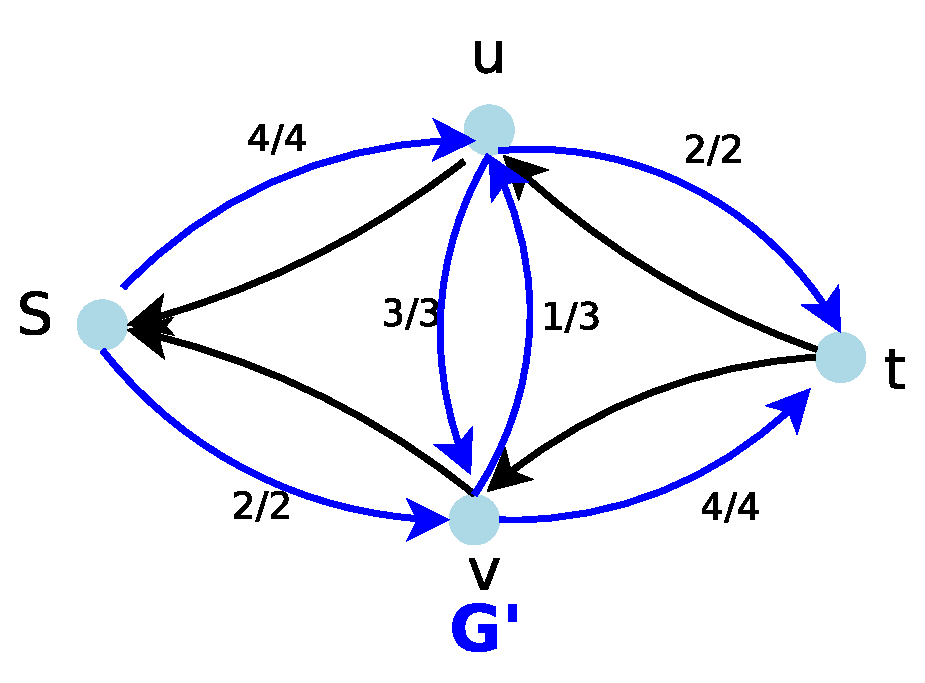
\includegraphics[width=1.5in] {L10-networkflowundirecteddirectedflow.eps}
\end{figure}

Note: the only trouble is the violation of capacity restriction: for edge $e=(u,v)$, $f(e)+f(e') = 4 > C(e) = 3$.
}

\frame{
\frametitle{ Step 3: revising flow to meet capacity restriction  }

\begin{figure}
 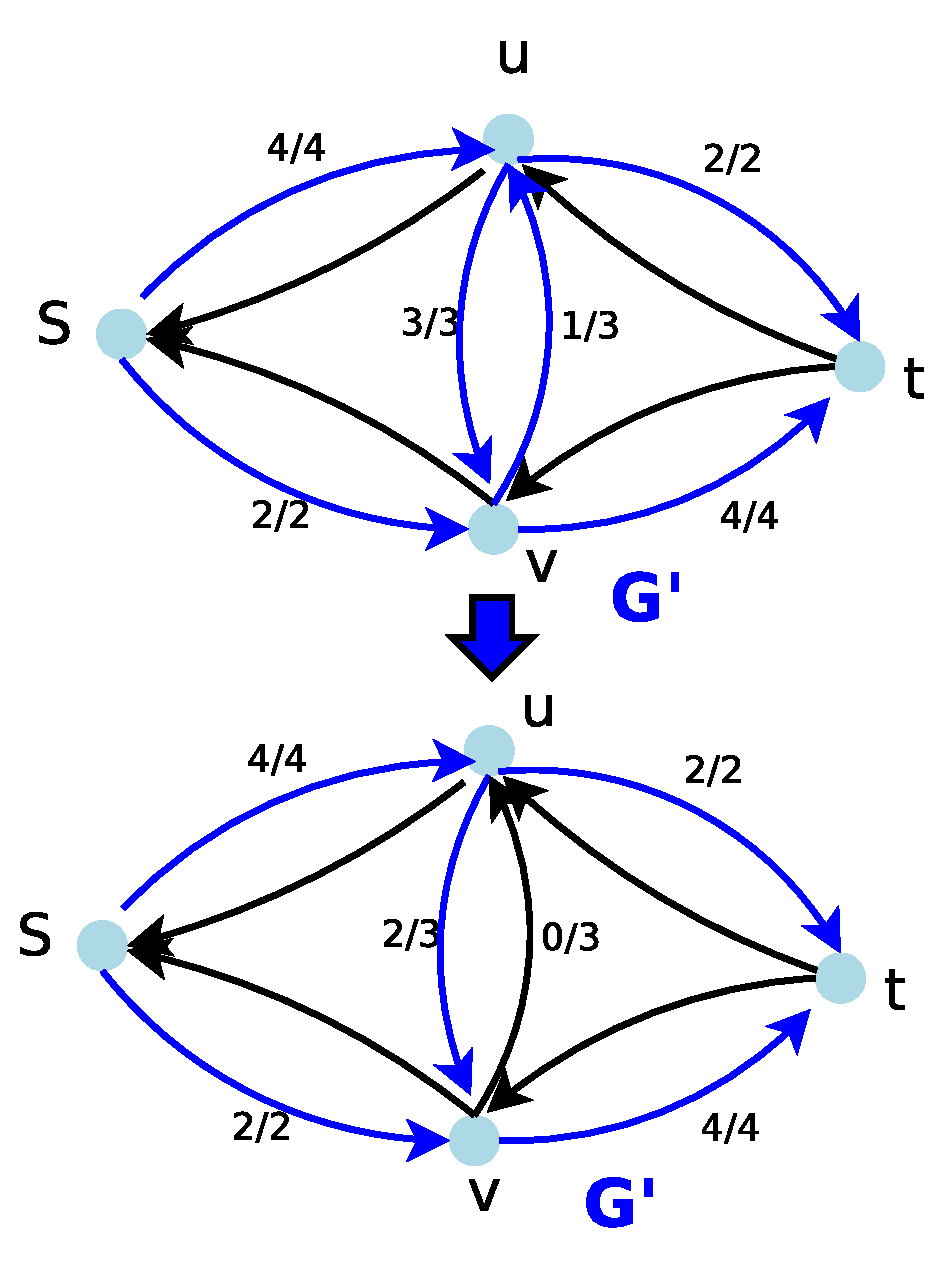
\includegraphics[width=1.8in] {L10-networkflowundirecteddirectedflowrevising.eps} 
\end{figure}
Note: for an edge violating capacity restriction, say $e=(u,v)$, the flow $f(e)$ and $f(e')$ were revised. 
} 
 
\frame{
\frametitle{ Correctness of revising flow }

\begin{small}
\begin{Theorem}
There exists a maximum flow $f$ for network $G$, where $f(u,v) = 0$ or $f(v,u)=0$. 
\end{Theorem}

\begin{figure}
 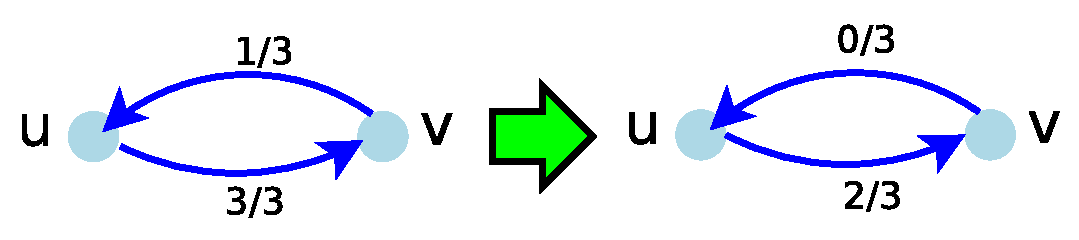
\includegraphics[width=1.9in] {L10-networkflowrevising.eps} 
\end{figure}

\begin{Proof}
\begin{itemize}
\item Suppose $f'$ is a maximum flow for undirected network $G'$, where $f'(u,v) > 0$ and $f'(v,u) > 0$. We change $f'$ to $f$ as follows: 
\item Let $\delta=\min\{ f'(u,v), f'(v,u) \}$. 
\item Define $f(u,v) = f'(u,v) - \delta$, and $f(v,u) = f'(v,u) - \delta$. We have $f(u,v) = 0$ or $f(v,u)=0$. 
\item It is obvious that both capacity restrictions and conservation restrictions hold.
\item $f$ has the same value to $f'$ and thus optimal. 
\end{itemize}
\end{Proof}
\end{small}
}

\frame{
\begin{block}{}
Extension 2: {\sc Circulation} problem with multiple sources and multiple sinks
\end{block}
}

\frame{
\frametitle{Extension 2: {\sc Circulation} problem with multiple sources and multiple sinks}

\begin{block}{}
{\bf INPUT: } \\ a network $G=<V, E>$, where each edge $e$ has a capacity $C(e) > 0$;  multi sources $s_i$ and sinks $t_j$. A sink $t_j$ has demand $d_j > 0$, while a source $s_i$ has supply $d_i$ ( described as a negative demand $d_i < 0$). \\ 
{\bf OUTPUT: } \\ a \textcolor{red}{\bf feasible circulation} $f$ to satisfy all demand requirements using the available supply, i.e., 
\begin{enumerate}
 \item Capacity restriction:  $0 \leq f(e) \leq C(e)$;
 \item Demand restriction:  $f^{in} (v) - f^{out} (v) = d_v$; 
\end{enumerate}
\end{block}
Note: For the sake of simplicity, we define $d_v=0$ for any node $v$ except for $s_i$ and $t_j$. Thus we have $\sum_i d_i = 0$, and denote  $D=\sum_{d_v >0 } d_v$ as  the \textcolor{red}{\bf total demands }.
} 

\frame{
\frametitle{ An example } 

\begin{figure}
 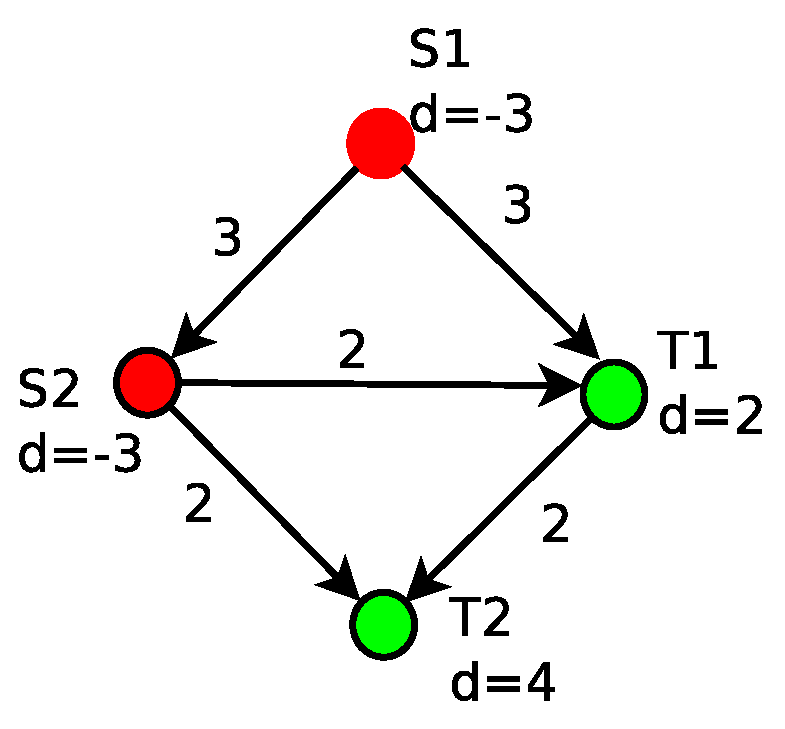
\includegraphics[width=1.3in] {L10-circulationexample.eps}
 %\caption{Two sources $s_1, s_2$ and two sinks $t_1, t_2$.}
\end{figure}


\textcolor{red}{Note: The differences between {\sc Circulation} and {\sc MultiCommodities} problem: } 
\begin{enumerate}
\begin{small}
\item  {\sc Circulation} problem: There is ONLY one type of commodity:  a sink $t_{i}$ can accept commodity from \textcolor{red}{\bf any} source. In other words, the combination of commodities from all sources constitutes the demand of $t_{i}$. 
 \item {\sc MultiCommodities} problem: There are multiple commodities, say transferring $food$ and $oil$ in the same network. Here $t_i$ (say demands $food$) accepts commodity $k_i$ from $s_i$ (say sending $food$) only. Linear programming is the only known polynomial-time algorithm for the {\sc MultiCommodities} problem.
 \end{small}
\end{enumerate}

%Note: 
}

\frame{
\frametitle{ Algorithm } 

Algorithm for circulation: 
  \begin{algorithmic}[1]
    \STATE Constructing an expanded network $G'$ via adding super source $S^*$ and super sink $T^*$; 
    \STATE Calculating the maximum flow $f$ for $G'$ by using Ford-Fulkerson algorithm;
    \STATE Return flow $f$ if the maximum flow value is equal to $D=\sum_{v: d_v > 0} d_v$. 
  \end{algorithmic}
}


\frame{
\frametitle{Step 1: constructing an expanded network $G'$}
 
{\bf Transformation:} constructing a network $G'$ through adding a super source $s^*$ to connect each $s_i$ with capacity $C(s^*,s_i)=-d_i$. Similarly, adding a super sink $t^*$ to connect to each $t_j$ with capacity $C(t_j,t^*)=d_j$. 

\begin{figure}
 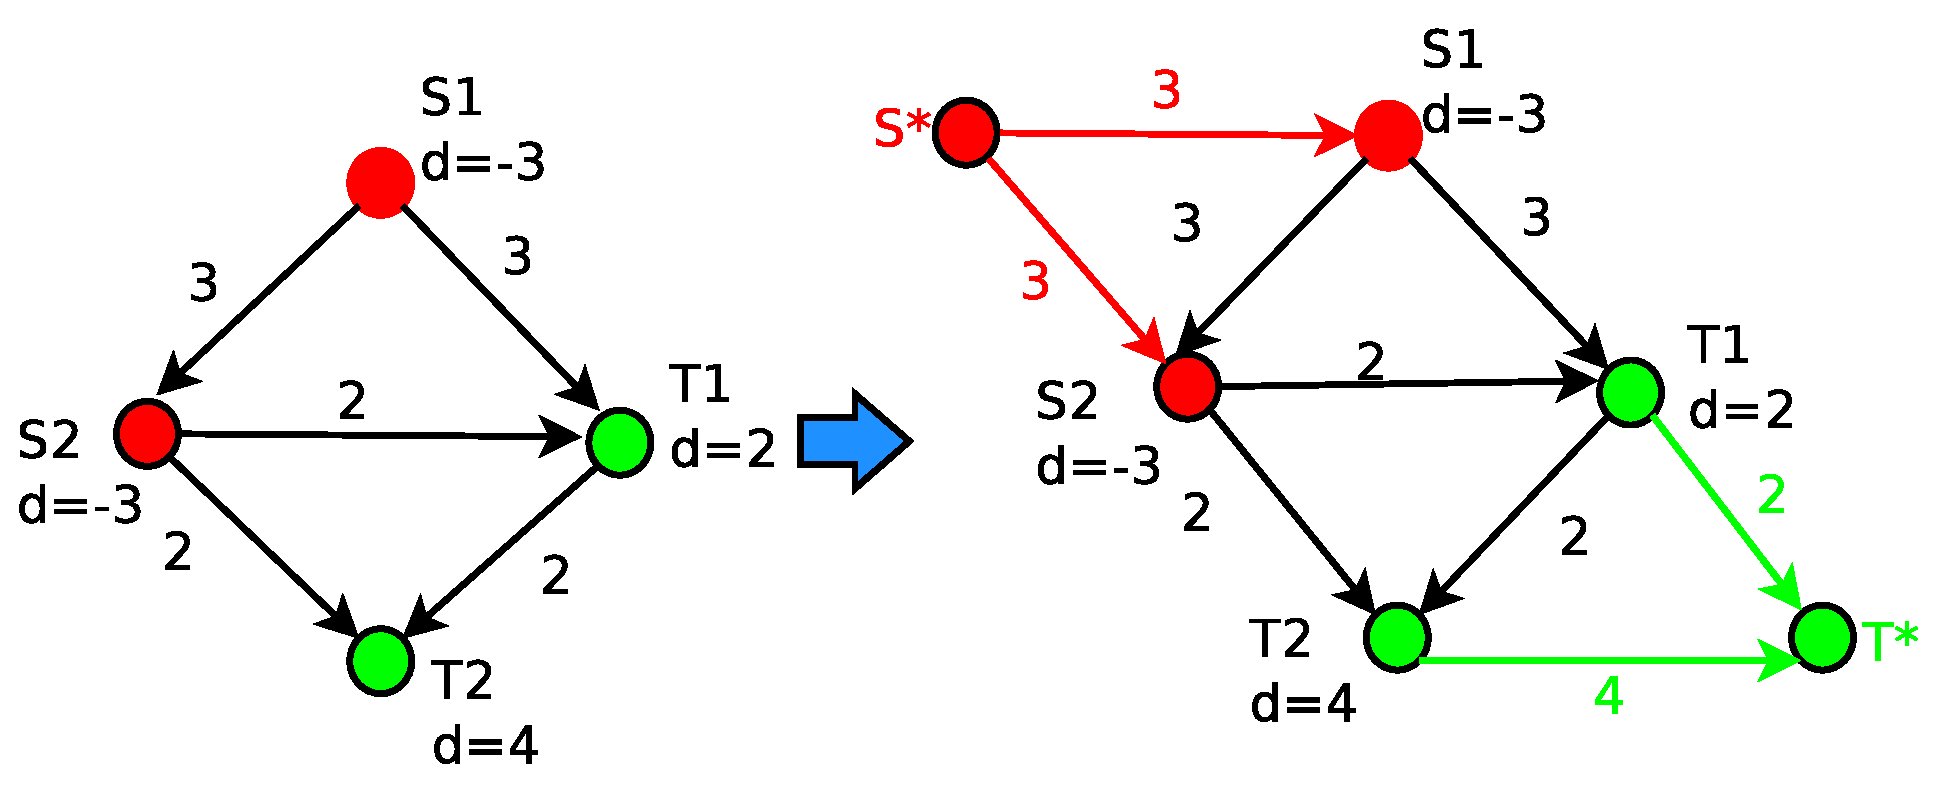
\includegraphics[width=3.5in] {L10-circulationexamplenetwork.eps}
\end{figure}
} 

\frame{
\frametitle{Step 2: calculating the maximum flow for $G'$}
 
\begin{figure}
 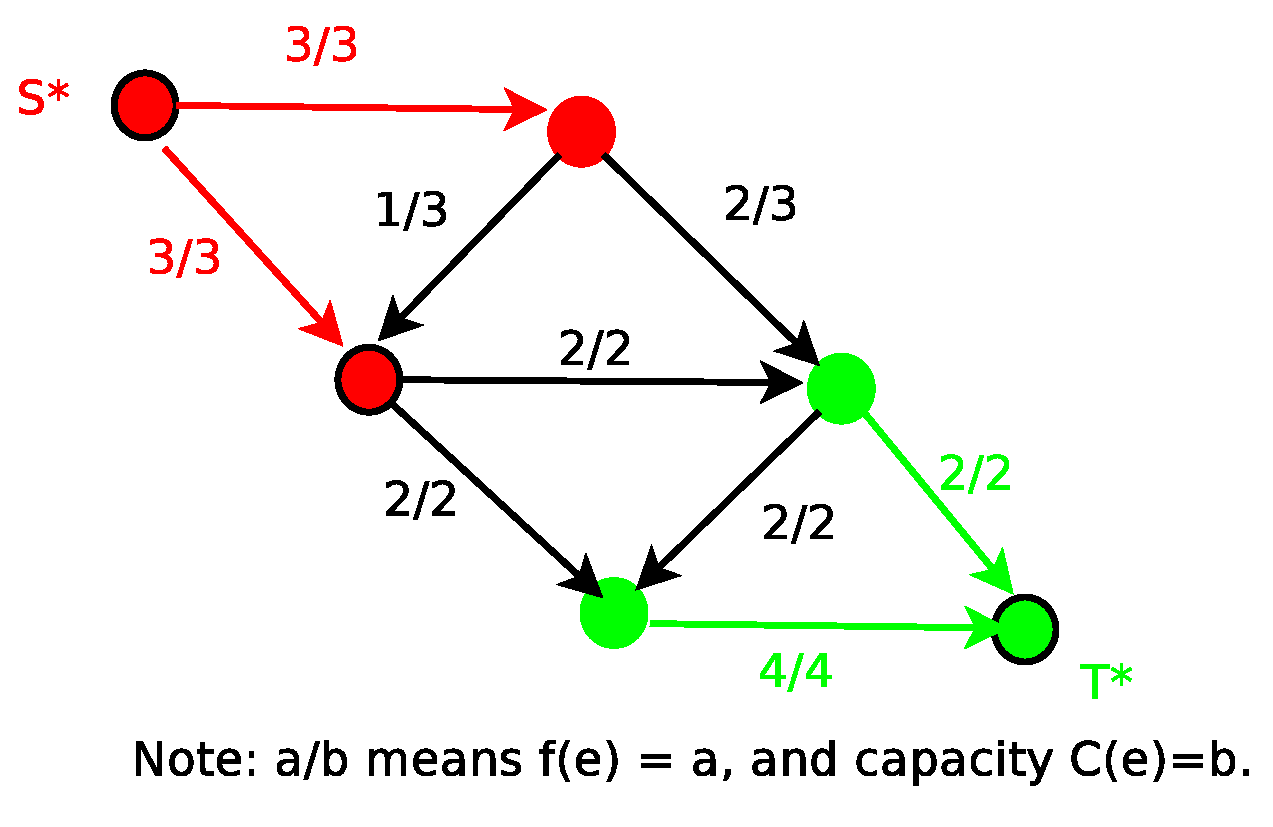
\includegraphics[width=3in] {L10-circulationtomaximumflow.eps}
\end{figure}
} 

\frame{
\frametitle{Step 3: checking the maximum flow for $G'$}
 
\begin{figure}
 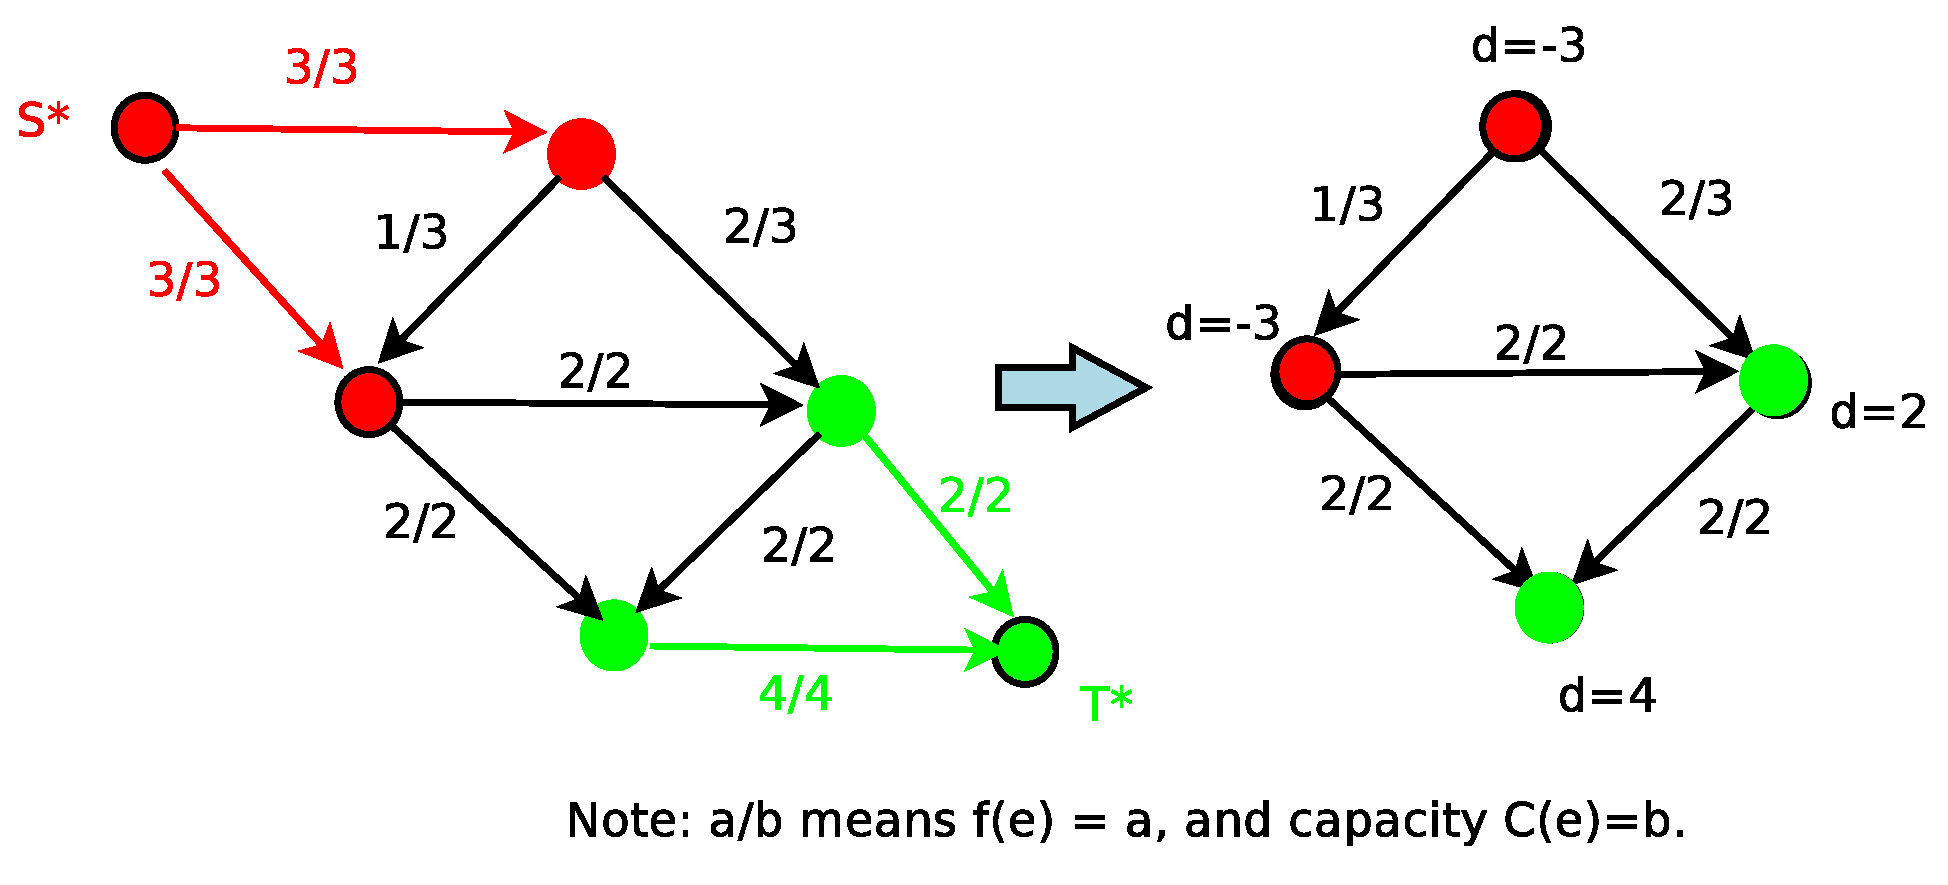
\includegraphics[width=3.5in] {L10-circulationtomaximumflowchecking.eps}
\end{figure}

The maximum flow value is $6 = \sum_{v, d_{v}>0} d_{v}$. Thus, we obtained a feasible solution to the original circulation problem. 
} 


\frame{
\frametitle{ Correctness }

\begin{Theorem}
There is a feasible solution to {\sc Circulation} problem iff the maximum $s^*-t^*$ flow in $G'$ is $D$. 
\end{Theorem}
\begin{Proof}
\begin{itemize}
 \item 
$\Leftarrow$ \\ 
  Simply removing all $(s^*,s_i)$ and $(t_j,t^*)$ edges. It is obvious that both capacity constraint and conservation constraint still hold for all $s_i$ and $t_j$.  \\

\item 
$\Rightarrow$  \\ 
We construct a $s^*-t^*$ flow and prove that it is a maximum flow: 
\begin{enumerate}
 \item 
Define a flow $f$ as follows: $f(s^*,s_i)=-d_i$ and $f(t_j, t^*)=d_j$. \\
\item 
Consider a special cut $(A,B)$, where $A=\{s^*\}$, $B=V-A$. 
\item 
We have $C(A,B)=D$. Thus $f$ is a maximum flow since it reaches the maximum value.
\end{enumerate}
\end{itemize}
 \end{Proof}
}

\frame{
\begin{block}{}
{Extension 3:  {\sc Circulation}  with lower bound for capacity}
\end{block}

} 

\frame{
\frametitle{Extension 3:  {\sc Circulation}  with lower bound of capacity}

\begin{block}{}
{\bf INPUT: } \\ a network $G=<V, E>$, where each edge $e$ has a capacity \textcolor{red}{upper bound} $C(e)$ and a \textcolor{red}{lower bound} $L(e)$;  multi sources $s_i$ and sinks $t_j$. A sink $t_j$ has demand $d_j > 0$, while a source $s_i$ has supply $d_i$ ( described as a negative demand $d_i < 0$). \\ 
{\bf OUTPUT: } \\  a feasible circulation $f$ to satisfy all demand requirements using the available supply, i.e., 
\begin{enumerate}
 \item Capacity restriction:  \textcolor{red}{$L(e) \leq f(e) \leq C(e)$};
 \item Conservation restriction:  $f^{in} (v) - f^{out} (v) = d_v$; 
\end{enumerate}
\end{block}
Note: For the sake of simplicity, we define $d_v=0$ for any node $v$ except for $s_i$ and $t_j$. Thus we have $\sum_i d_i = 0$, and define $D=\sum_{d_v >0 } d_v$ be the {\it total demands }.

}


\frame{
\frametitle{ An example }
\begin{figure}
 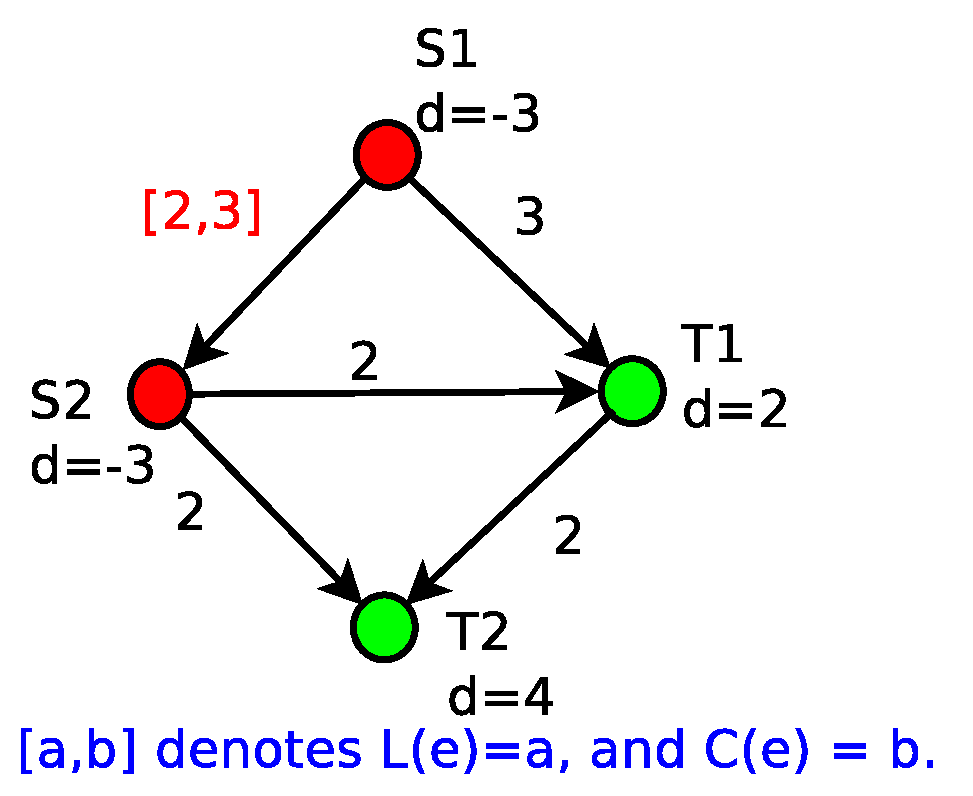
\includegraphics[width=2in] {L10-lowerboundcirculationexample.eps}
\end{figure}

Advantages of lower bound: By setting lower bound $L(e)>0$, we can force edge $e$ to be used by flow, e.g. edge $(s_{1}, s_{2})$ should be used in the flow. 
}

\frame{
\frametitle{ Algorithm } 

Algorithm for circulation with lower-bound for capacity
  \begin{algorithmic}[1]
    \STATE Building \textcolor{red}{\bf an initial flow} $f_0$ by setting $f_0(e) = L(e)$ for $e=(u,v)$; 
    \STATE Solving a new circulation problem for $G'$ without capacity lower bound. Specifically, $G'$ was made by revising an edge $e=(u,v)$ with lower bound capacity:
     \begin{enumerate}
     \item nodes: $d'_u = d_u + L(e)$, $d'_v = d'_v - L(e)$,
     \item edge:  $L(e) = 0$, $C(e) = C(e) - L(e)$.
     \end{enumerate}
     Denote $f'$ as a feasible circulation to $G'$.  
    \STATE Return $f=f'+f_0$. 
   \end{algorithmic}
}

\frame{
\frametitle{ Step 1: Building an initial flow $f_0$ } 

\begin{figure}
 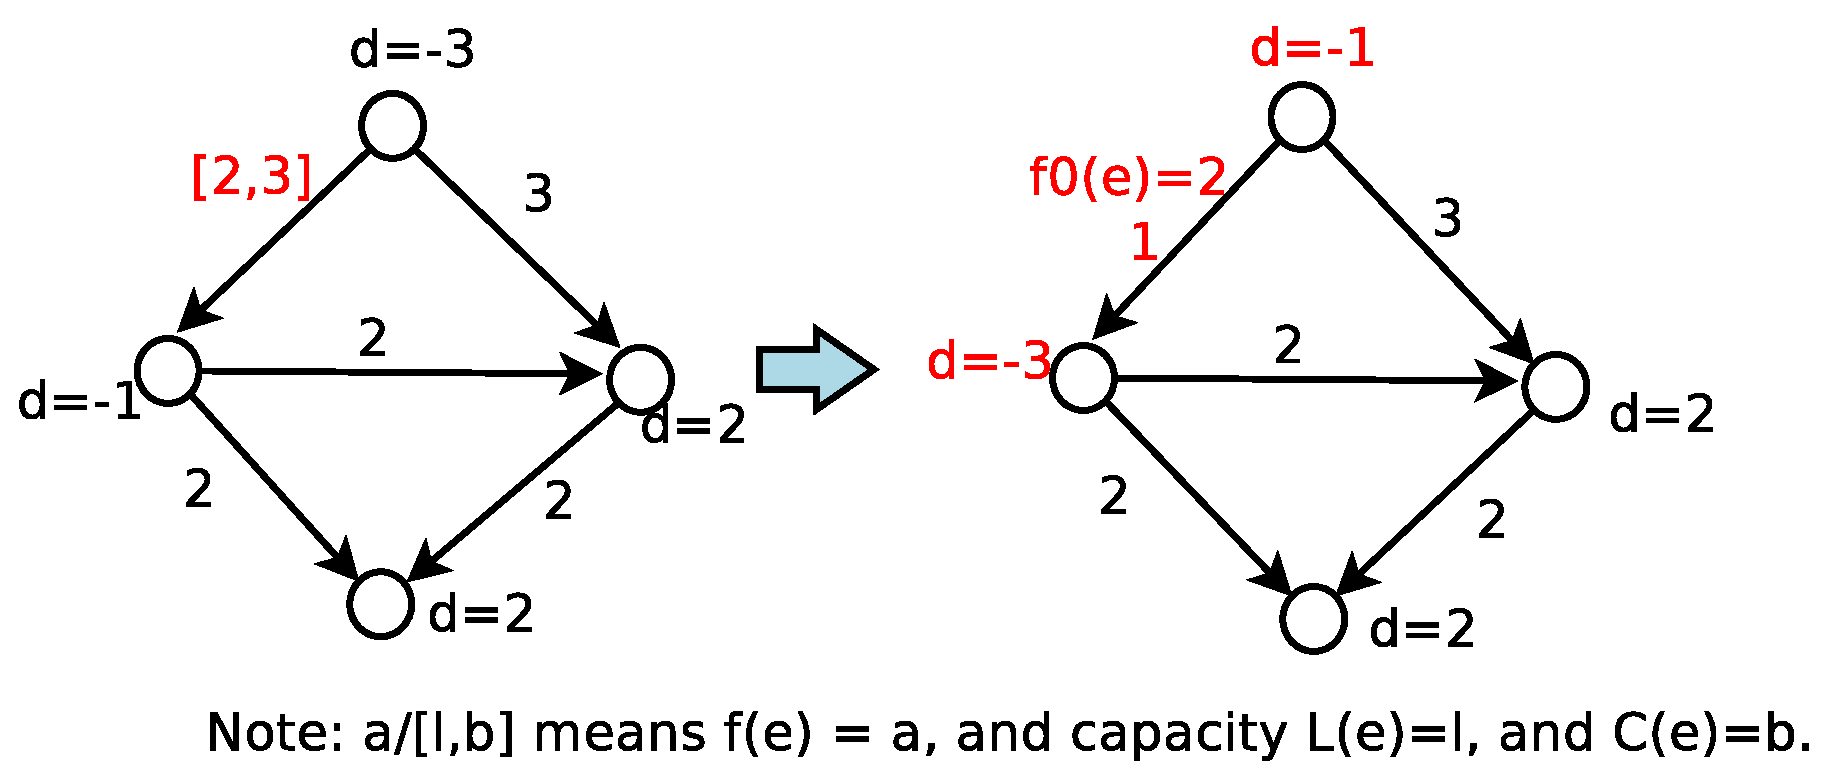
\includegraphics[width=3.8in] {L10-lowerboundcirculationstep1.eps}
\end{figure}
}

\frame{
\frametitle{ Step 2: Solving the new circulation problem } 

\begin{figure}
 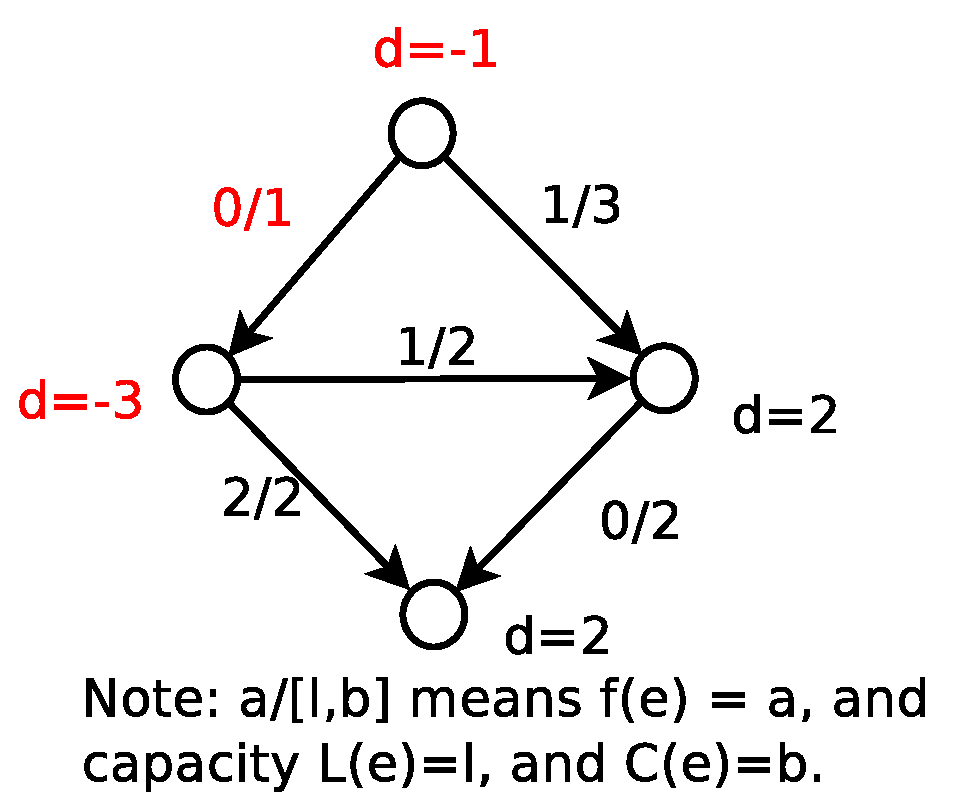
\includegraphics[width=1.8in] {L10-lowerboundcirculationstep2.eps}
\end{figure}
We found a feasible circulation $f'$ for the network $G'$. 
}

\frame{
\frametitle{ Step 3: Adding $f_0$ and $f'$ } 

\begin{figure}
 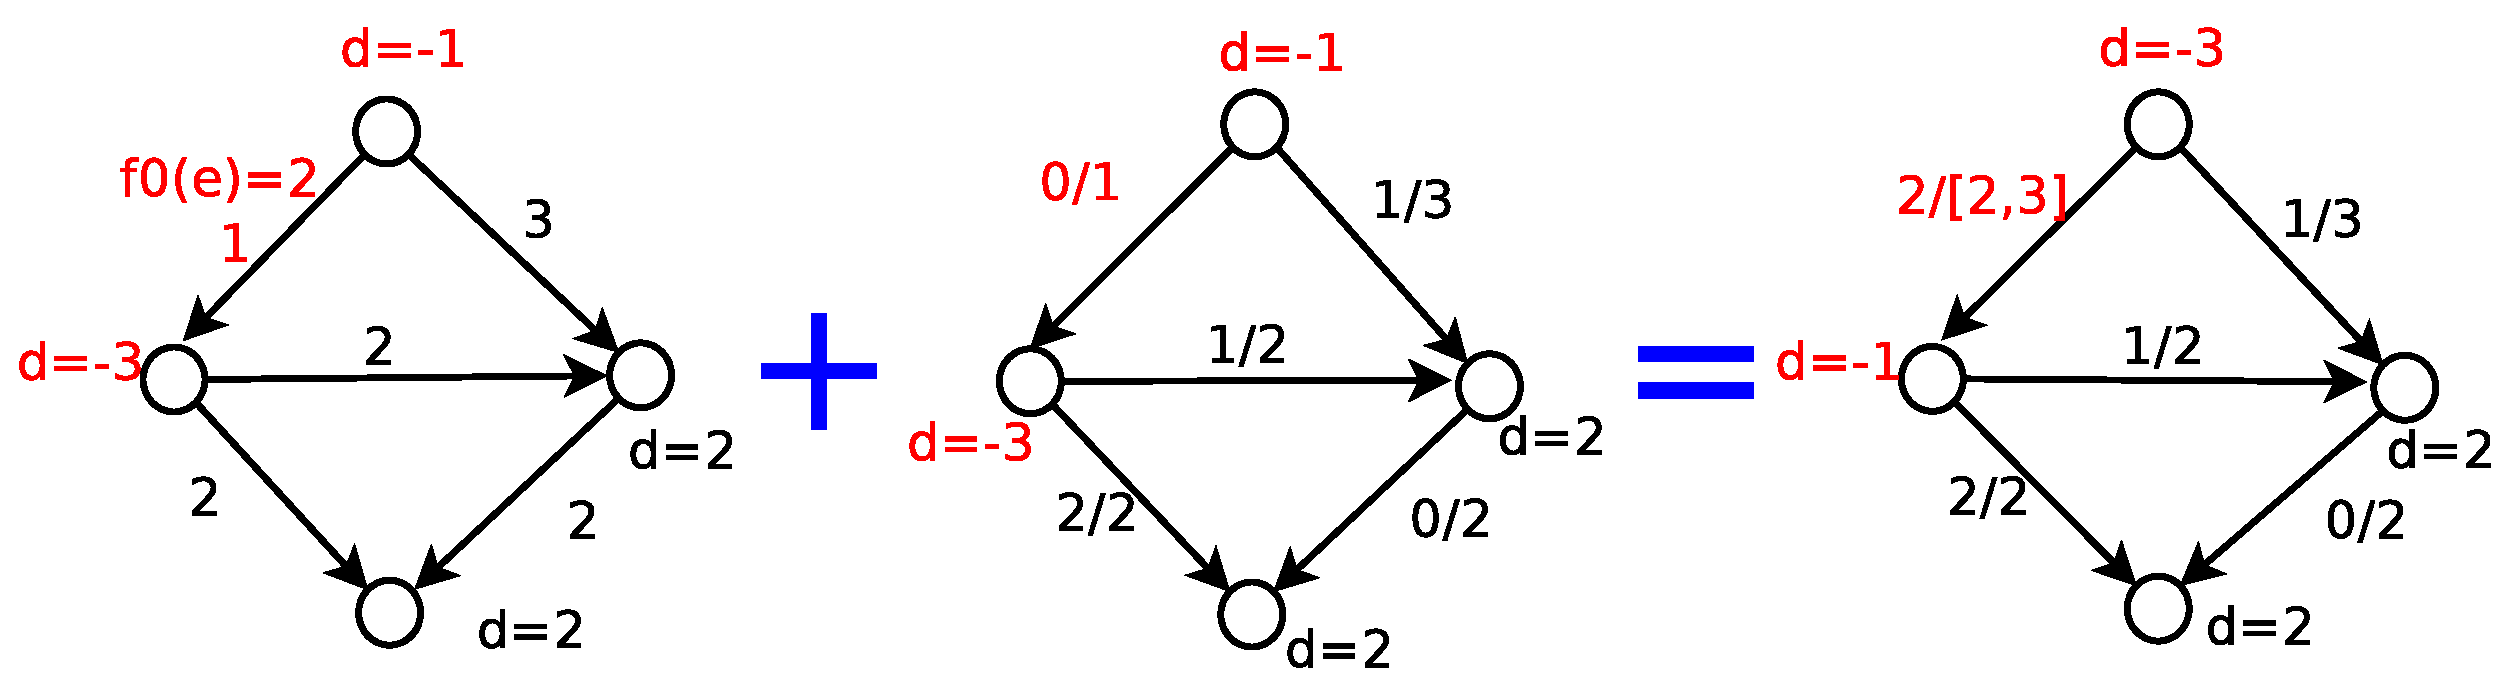
\includegraphics[width=4.5in] {L10-lowerboundcirculationstep3.eps}
\end{figure}

We get $f$ to the original problem as: $f=f_0 + f'$.
}


%\frame{
%\frametitle{ Example 2 } 
%
%\begin{figure}
% 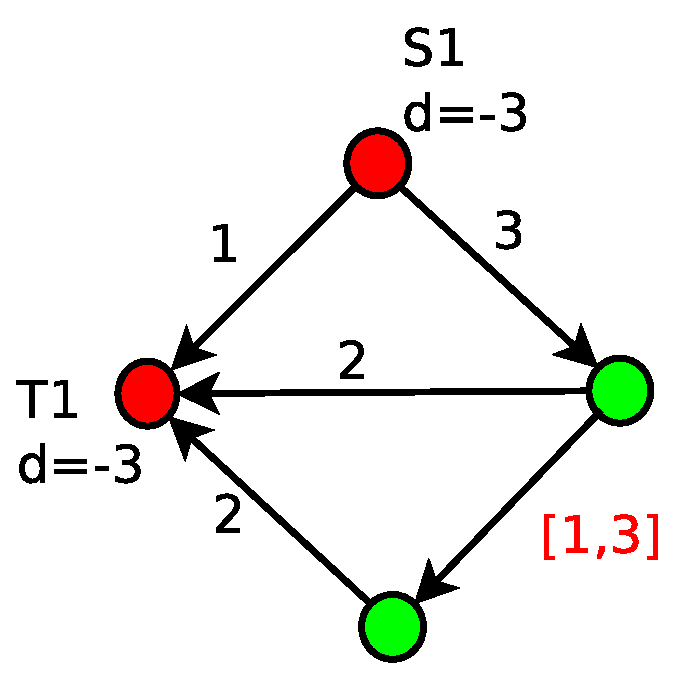
\includegraphics[width=1.8in] {L10-lowerboundcirculationexample2.eps}
%\end{figure}
%}
%
%
%\frame{
%\frametitle{ Step 1: Building an initial flow $f_0$ } 
%
%\begin{figure}
% 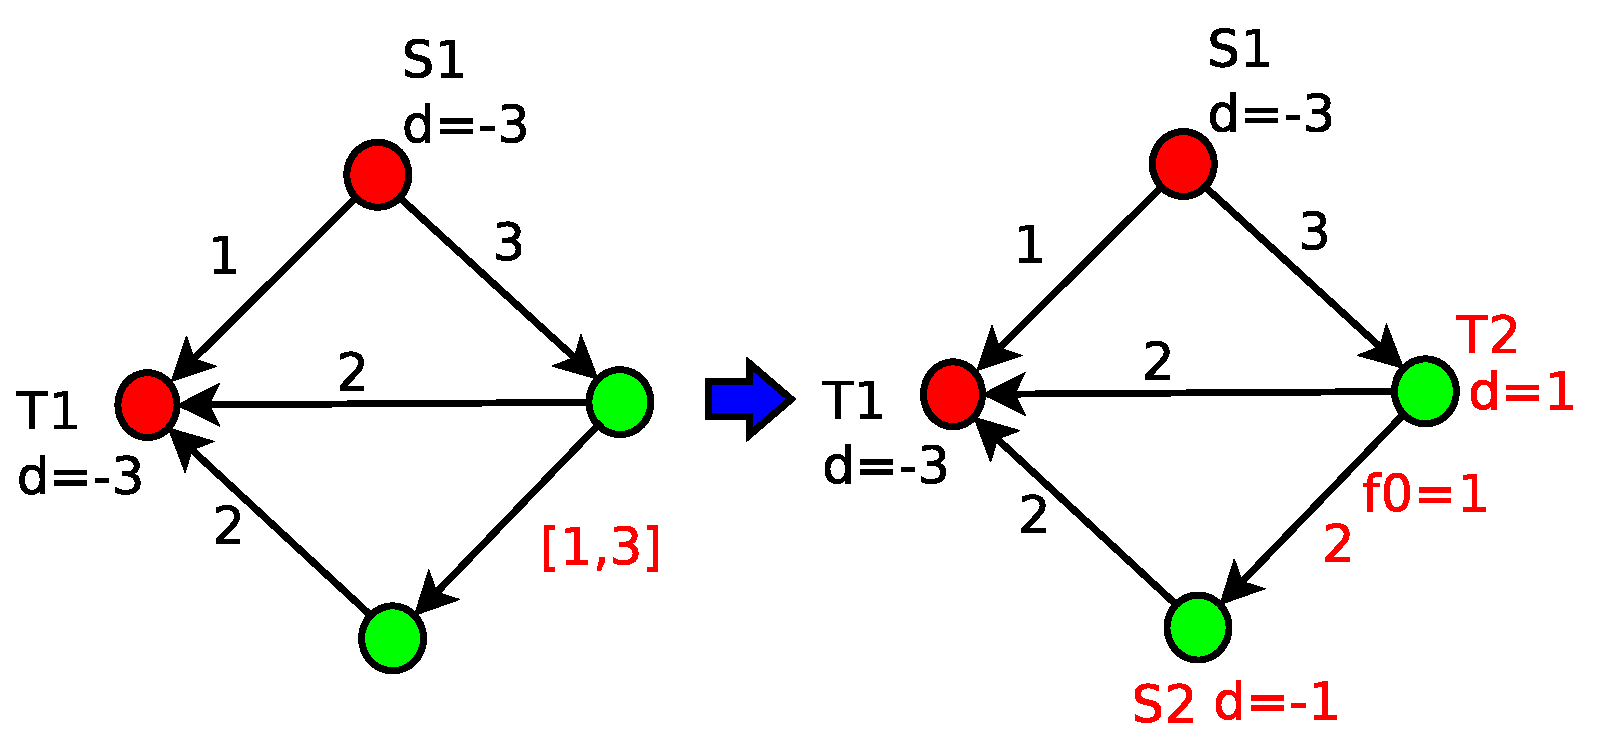
\includegraphics[width=3.8in] {L10-lowerboundcirculationexample2step1.eps}
%\end{figure}
%}
%
%\frame{
%\frametitle{ Step 2: Solving the new circulation problem } 
%
%\begin{figure}
% 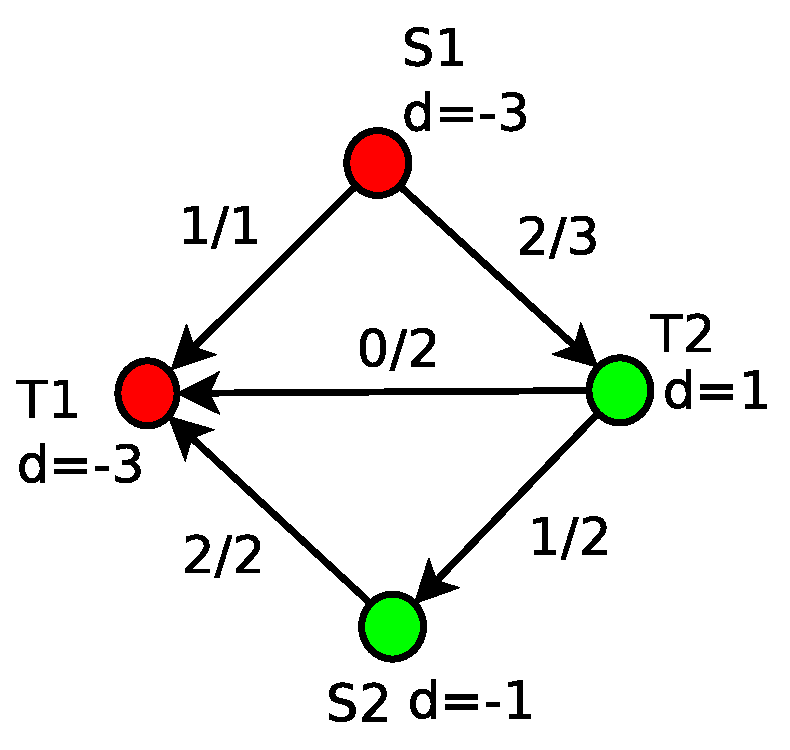
\includegraphics[width=1.8in] {L10-lowerboundcirculationexample2step2.eps}
%\end{figure}
%We found a feasible circulation $f'$ for the network $G'$. 
%}
%
%\frame{
%\frametitle{ Step 3: Adding $f_0$ and $f'$ } 
%
%\begin{figure}
% 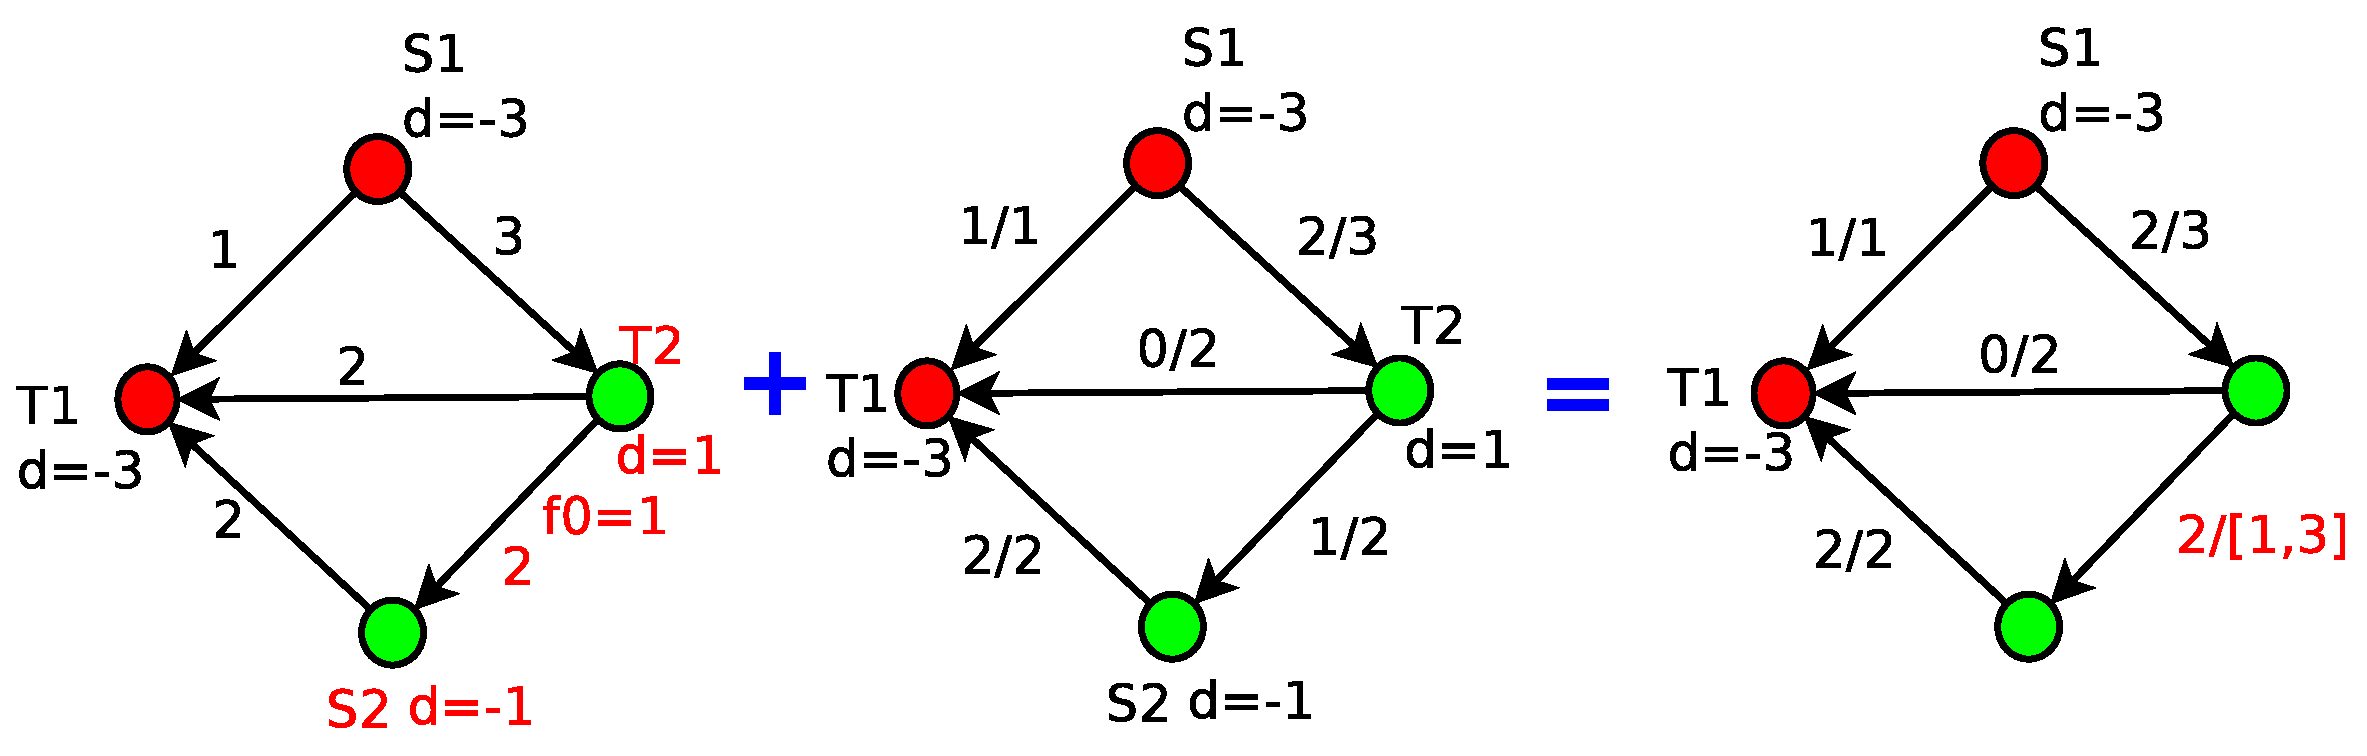
\includegraphics[width=4.5in] {L10-lowerboundcirculationexample2step3.eps}
%\end{figure}
%
%We get $f$ to the original problem as: $f=f_0 + f'$.
%}




% \frame{
% \frametitle{Extension 3: Lower bound of capacity cont'd}
% 
% Reduction: 
% \begin{enumerate}
% \item 
% We build an initial circulation $f_0$ by setting $f_0(e) = L(e)$. 
% \item 
% Next we improve $f_0$ to a circulation $f'$ through solve another {\sc Circulation} problem: construct a network $G'$ without lower bound restrictions on capacity, and demands $d'_v = d_v - L(w,v)$. \\
% \end{enumerate}
% 
% \begin{figure}
%  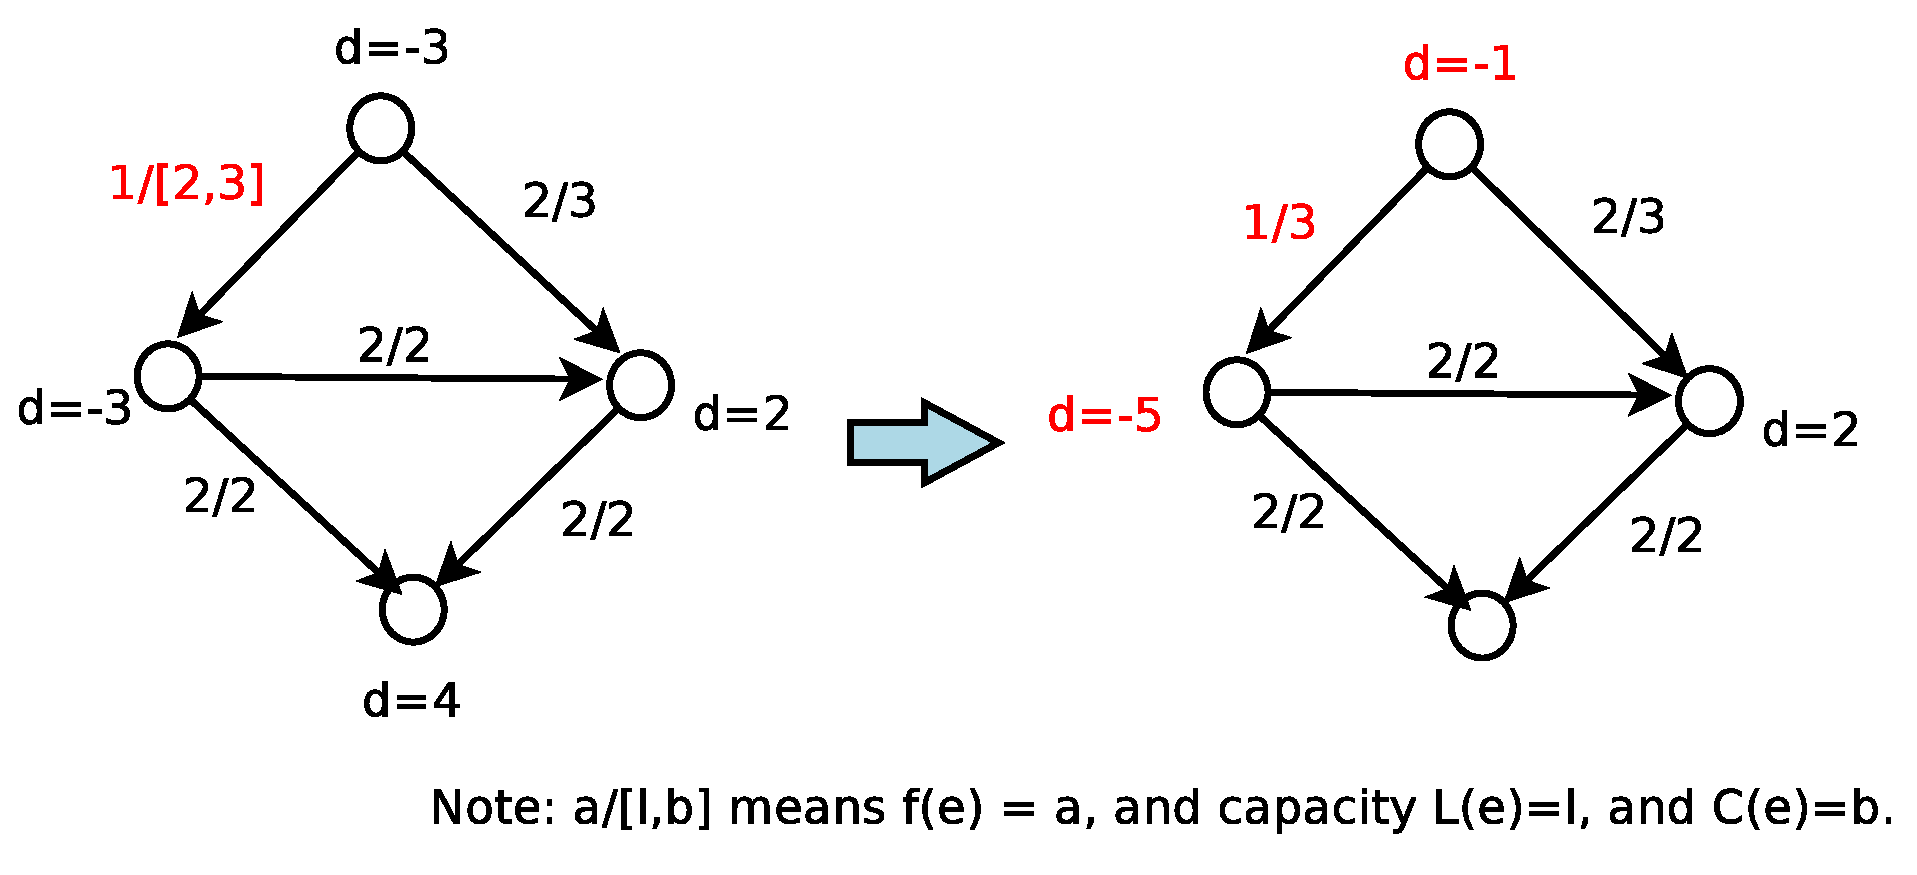
\includegraphics[width=2.8in] {L10-lowerboundcirculation.eps}
% \end{figure}
% } 


\frame{
\frametitle{Correctness }


\begin{Theorem}
 There is a circulation $f$ to $G$ (with lower bounds) iff there is a circulation $f'$ to $G'$ (without lower bounds). 
\end{Theorem}
\begin{Proof}
\begin{itemize}
\item Define $f'(e) = f(e)+L_e$. 
\item It is easy to verify both capacity constraints and conservation constraints hold. 
\end{itemize}
\end{Proof}
}

\frame{
\begin{block}{}
{ Extension 4: {\sc Minimum Cost Flow} problem } 
\end{block}
} 

\frame{
\frametitle{ Extension 4: {\sc Minimum Cost Flow} } 

\begin{block}{}
{\bf INPUT: }  \\ a network $G=<V, E>$, where each edge $e$ has a capacity $C(e) > 0$, and \textcolor{red}{a cost $w(e)$} for transferring a unit through edge $e$. Two special node: source $s$ and sink $t$. A flow value $v_0$.  \\ 
{\bf OUTPUT: } \\ to find a circulation $f$ with flow value $v_0$ and the cost is minimized. 
\end{block}
} 

\frame{
\frametitle{ An example } 

\begin{figure}
        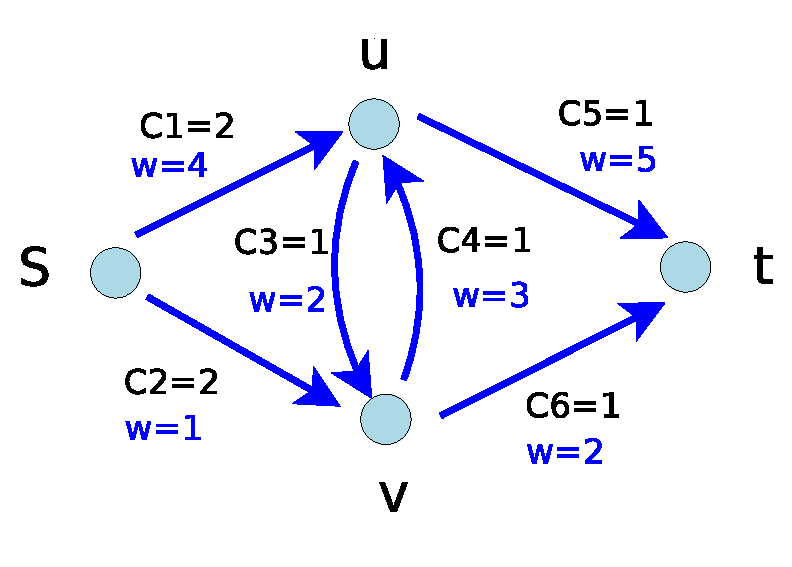
\includegraphics[width=1.8in]{L10-mincostflowexample.eps}
\end{figure}
\begin{itemize}
\item 
Objective: how to transfer $v_{0}=2$ units commodity from $s$ to $t$ with the minimal cost?
\item 
Basic idea: the cost $w_{e}$ makes it difficult to find the minimal cost flow by simply expanding $G$ to $G'$ as we did for the {\sc Circulation} problem. Then we return  to the primal\_dual idea.  
\end{itemize}
}

\frame{
\frametitle{ Primal\_Dual technique: LP formulation } 
\begin{figure}
        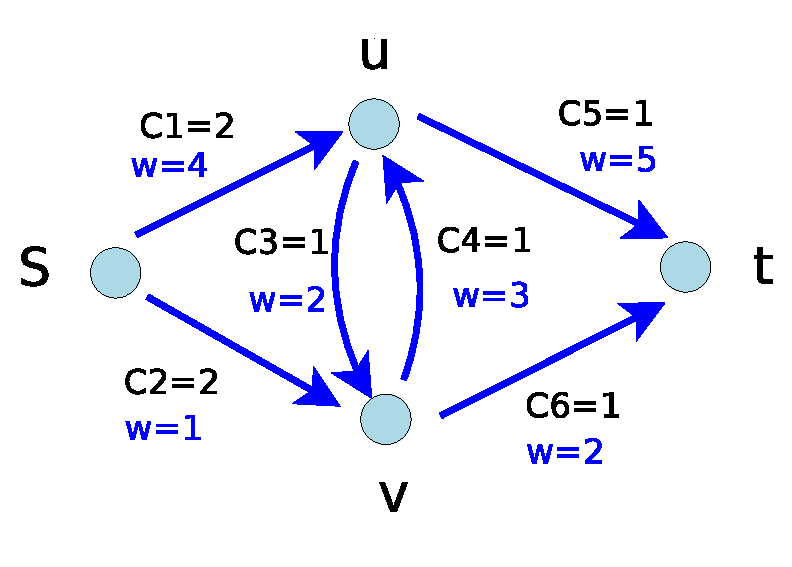
\includegraphics[width=1.5in]{L10-mincostflowexample.eps}
\end{figure}

\[
\begin{array}{rrrrrrrllllll}
\textcolor{red}{ \min } &4y_1&+ y_2&+ 2y_3&+3y_4&+5y_5&+2y_6 &         &  \\
 s.t. & y_1 &+ y_2&    &    &      &      & \textcolor{red}{=}  2 &  \text{node } s \\
      &     &     &    &    &  -y_5 &-y_6 & \textcolor{red}{=}  -2 &  \text{node } t\\
      & -y_1 &     &+y_3&-y_4&+y_5 &      & \textcolor{red}{=}  0 &  \text{node } u\\
      &     & -y_2&-y_3&+y_4&   &+y_6 & \textcolor{red}{=}  0 &  \text{node } v\\
      &     &     &    &    &      &  y_i & \leq  C_i & \\
      &     &     &    &    &      &  y_i & \geq  0 & \\
\end{array} \nonumber
\] 
Intuition: $y_{i}$ denotes the flow on edge $i$. 
}



\frame{
\frametitle{ Primal\_Dual technique: Dual form D } 
\[
\begin{array}{rrrrrrrllllll}
\textcolor{red}{ \max } &-4y_1&-y_2&-2y_3&-3y_4&-5y_5&-2y_6 &         &   \\
 s.t. & y_1 &+y_2&    &    &      &      & \textcolor{red}{\leq}  2 &  \text{node } s  \\
      &     &     &    &    &-y_5 &-y_6 & \textcolor{red}{\leq}  -2 &  \text{node } t  \\
      &-y_1 &     &+y_3&-y_4&+y_5 &      & \textcolor{red}{\leq}  0 &  \text{node } u  \\
      &     &-y_2&-y_3&+y_4&   &+y_6 & \textcolor{red}{\leq} 0 &  \text{node } v  \\
      &     &     &    &    &      &  y_i & \leq  C_i &  &\\
      &     &     &    &    &      &  y_i & \geq  0 &  &\\
\end{array} 
\] 

Rewrite the LP into standard DUAL form via:   
\begin{itemize}
 \item Objective function: using $\max$ instead of $\min$. 
 \item Constraints:  Simply replacing  ``$=$'' with ``$\leq$''.  (Why? Notice that if all inequalities were  satisfied, they should be equalities. For example, inequalities (2), (3) and (4) force $y_{1} + y_{2} \geq 2$, thus change $\leq$ into $=$ for inequality (1). So do other inequalities. 
\end{itemize}
}

\frame{
\frametitle{Finding a valid circulation with value $v_{0}$ first. } 

\begin{itemize}
\item We need to find a valid circulation with value $v_{0}=2$ first. 
\item This is easy: {\sc Circulation} problem. 
\item Thus we have a feasible solution to $D$. 
\end{itemize}

}


\frame{
\frametitle{ Primal\_Dual technique: DRP } 

\begin{small}
\[
\begin{array}{rrrrrrrlllllll}
 \max &-4y_1&-y_2&-2y_3&-3y_4&-5y_5&-2y_6 &         &  \\
 s.t. & y_1 &+y_2&    &    &      &      & \leq  0 &  \text{node } s \\
      &     &     &    &    & y_5 &+y_6 & \leq  0 &  \text{node } t\\
      & y_1 &     &-y_3&+y_4&-y_5 &      & \leq  0 &  \text{node } u\\
      &     &  y_2&+y_3&-y_4&  &-y_6 & \leq  0 &  \text{node } v\\
      &     &     &    &    &      &  y_i & \leq  0 & \text{for full arc}\\
      &     &     &    &    &      & -y_i & \leq  0 & \text{for empty arc}\\
      &     &     &    &    &      &  y_i & \leq  1 & \text{for any arc}\\
\end{array} \nonumber
\] 
\end{small}
Recall the rules to construct DRP from D:
\begin{itemize}
 \item Replacing the right hand items with $0$. 
 \item Removing the constraints not in $J$ ($J$ contains the constraints in $D$ where $=$ holds).
 \item Adding constraints $y_{i}  \geq -1$ for any arcs.  
\end{itemize}
}

\frame{
\frametitle{ Solving DRP: combinatorial technique rather than simplex } 

\begin{Definition}[{\bf Cycle flow}]
A flow $f$ is called \textcolor{red}{\bf cycle flow } if input equal output for any node (including $s$ and $t$). 
\end{Definition}

\begin{itemize}
 \item Suppose we have already obtained a flow for network $N$. 
 \item Solving the corresponding DRP is essentially finding a cycle in a new network $N'(f)$, which  is constructed as follows: 
\begin{enumerate}
\begin{small}
 \item For each edge $e=(u,v)$ in $N$, two edges $e=(u,v)$ and $e'=(v,u)$ were introduced to $N'(f)$;
 \item The capacities for $e$ and $e'$ in $N'(f)$ are set as $C(e)-f(e)$ and $-f(e)$, respectively; 
 \item The costs are set as $w(e')=-w(e)$;
 \end{small}
\end{enumerate}
\begin{figure}
 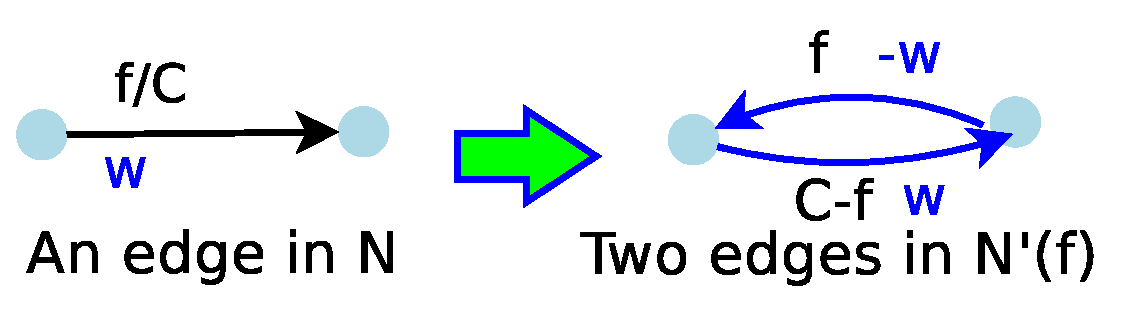
\includegraphics[width=2.5in] {L10-mincostflowNN.eps}
\end{figure}
\end{itemize}

}


\frame{
\frametitle{ Minimum cost flow algorithm [M. Klein 1967] } 

\begin{Theorem}
 $f$ is the minimum cost flow in network $N$ $\Leftrightarrow$ network $N'(f)$ contains no cycle with negative cost. 
\end{Theorem}
\begin{Proof}
$f$ is the minimum cost flow in network $N$ \\
$\Leftrightarrow$  The optimal solution to $DRP$ is $0$. \\
$\Leftrightarrow$  $N'(f)$ has no cycle flow with negative cost. \\
$\Leftrightarrow$  $N'(f)$ has no cycle with negative cost. 
\end{Proof}
Intuition: Suppose that we have obtained a cycle in $N'(f)$. Pushing a unit flow along the cycle leads to a cycle flow (denoted as $\overline{f}$). Then $f+\overline{f}$ is also a flow for the original network $N$. 
} 

\frame{
\frametitle{ Minimum cost flow algorithm } 

Klein algorithm 
  \begin{algorithmic}[1]
    \STATE Finding a flow $f$ with value $v_0$ using maximum-flow algorithm, say Ford-Fulkerson; 
    \WHILE { $N'(f)$ contains a cycle $C$ with negative cost } 
    \STATE Denote $b$ as the bottleneck of cycle $C$. 
    \STATE Define $\overline{f}$ as the unit flow along $C$. 
    \STATE $f=f+b \overline{f}$; 
    \ENDWHILE
    \RETURN $f$.
  \end{algorithmic}
Note: 
\begin{enumerate}
 \item The cost of flow decreases as iteration proceeds, while the flow value keeps constant.
 \item The cycle with negative cost can be found using Bellman-Ford algorithm.
\end{enumerate}

}

\frame{
\frametitle{ Example: Step 1} 
Initial flow $f_0$: flow value $2$, flow cost: $17$. 
\begin{figure}
 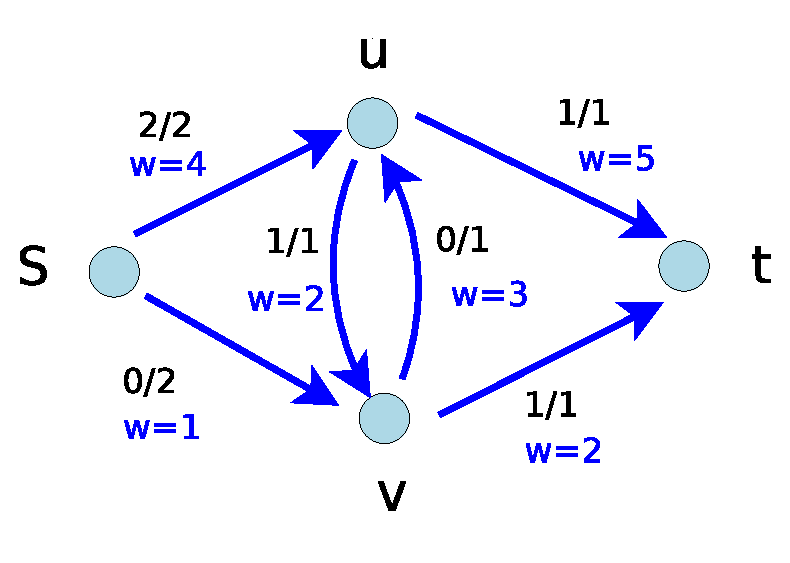
\includegraphics[width=1.5in] {L10-mincostflowexamplestep1.eps}
\end{figure}

New network $N'(f)$: 
\begin{figure}
 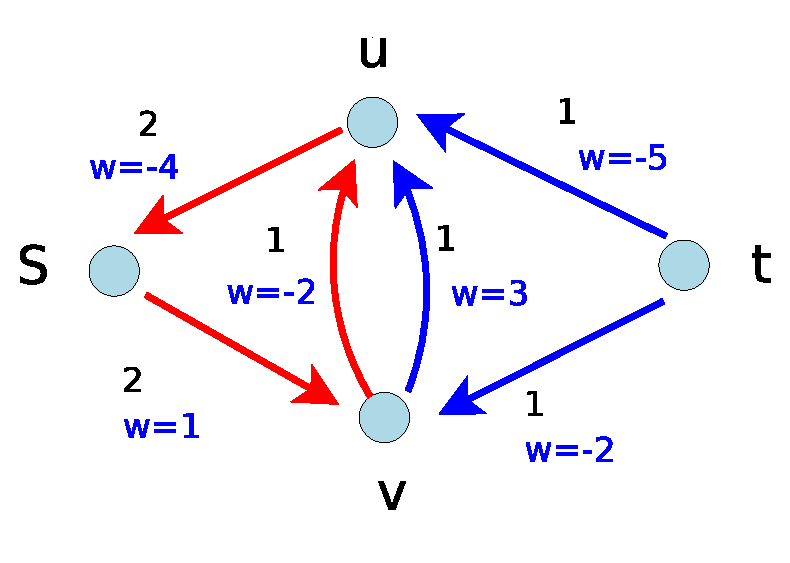
\includegraphics[width=1.5in] {L10-mincostflowexamplestep1N.eps}
\end{figure}

Negative cost cycle: $s\rightarrow v\rightarrow u\rightarrow s$ (in red). Cost: $-5$. 
}

\frame{
\frametitle{ Example: Step 2} 
$f=f+\overline{f}$: flow value $2-0=2$, flow cost: $17-5=12$.
\begin{figure}
 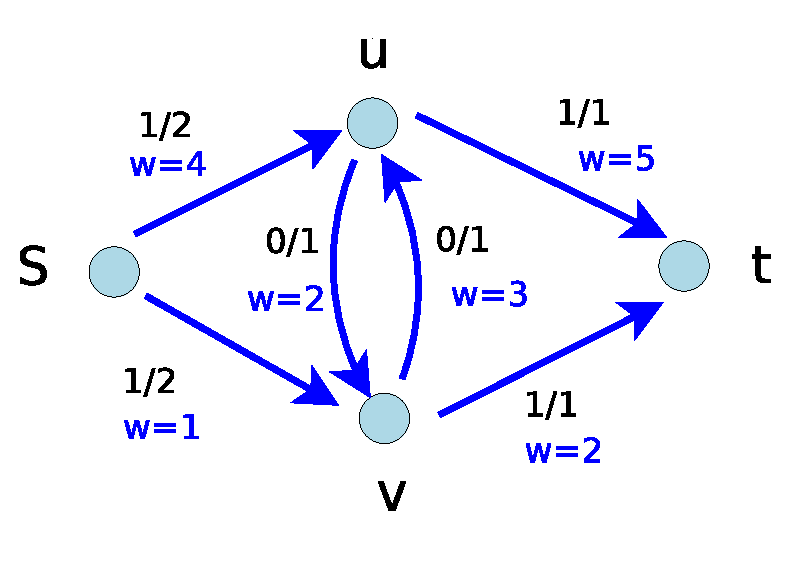
\includegraphics[width=1.5in] {L10-mincostflowexamplestep2.eps}
\end{figure}

New network $N'(f)$: 
\begin{figure}
 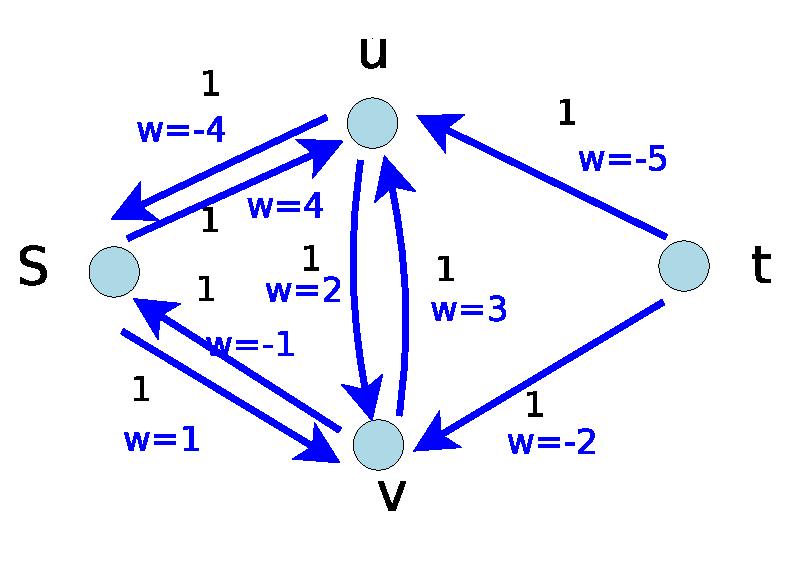
\includegraphics[width=1.5in] {L10-mincostflowexamplestep2N.eps}
\end{figure}

Negative cost cycle: cannot find. Done! 
}

\frame{
\frametitle{Extension: Hitchcock {\sc Transportation} problem 1941 }

\begin{block}{}
{\bf INPUT: } $n$ sources $s_1, s_2, ..., s_n$ and $n$ sinks $t_1, t_2, ..., t_n$. Source $s_i$ has supply $a_i$, and a sink $t_j$ has demand $b_j$. The cost from $s_i$ to $t_j$ is $c_{ij}$. 
 
{\bf OUTPUT: } arrange a schedule to minimize cost. 
\end{block}

Note: 

\begin{enumerate}
 \item Frank L. Hitchcock formulated the{\sc Transportation} problem in 1941. This problem is equivalent to {\sc Minimum Cost Flow problem} [Wagner, 1959].
 \item In 1956, L. R. Ford Jr. and D. R. Fulkerson proposed a "labeling" technique to solve the transportation problem. This algorithm is considerably more efficient than simplex algorithm. See "Solving the Transportation Problem" by L. R. Ford Jr. and D. R. Fulkerson. 
 \item If $c_{ij}=0/1$, then Hitchcock problem turns into assignment problem. 
\end{enumerate}

}


\frame{
\begin{block}{}
{Applications of {\sc MaximumFlow} problem } 
\end{block}

} 

\frame{
\frametitle{Applications of {\sc MaximumFlow} problem }
\ \\
\begin{block}{}
Formulating a problem into {\sc MaximumFlow} problem: 
\begin{enumerate}
 \item We should define a \textcolor{red}{\bf network}  first. Sometimes we need to construct a graph from the very scratch.
\item Then we need to define  \textcolor{red}{\bf weight for edges}. Sometimes we need to move the weight on nodes to edges.
 \item How to define  \textcolor{red}{\bf  source $s$ and sink $t$ }? Sometimes super source $s^*$ and $t^*$ are needed. 
\item Finally we need to prove that  \textcolor{red}{\bf max-flow} (finding paths, matching) or  \textcolor{red}{\bf  min-cut} (partition nodes) is what we wanted.
\end{enumerate}
Note: most problems utilize the property that there exists a maximum integer-valued flow iff there exists a maximum flow. 
\end{block}
}

\frame{
\begin{block}{}
 Paradigm 1: Partition a set 
\end{block}
}

\frame{
\frametitle{ Problem 1:  {\sc ImageSegmentation} problem }
\begin{block}{}
{\bf INPUT:} \\ Given an image in pixel map format. The pixel $i, i\in P$ has a probability to be foreground $f_i$ and the probability to be background $b_i$; in addition, the likelihood that two neighboring pixels $i$ and $j$ are similar is $l_{ij}$; \\
{\bf GOAL: } \\ to identify foreground out of background. Mathematically, we want a partition  $P=F\cup B$, such that $Q(F, B) = \sum_{i\in F} f_i + \sum_{j\in B} b_i + \sum_{i \in F}\sum_{j \in N(i)\cap F} l_{ij} + \sum_{i \in B}\sum_{j \in N(i)\cap B} l_{ij}$ is maximized.   
\end{block}

 \begin{figure}
        
\includegraphics[width=1.0in]{L10-image-Einstein.png}
 \end{figure}
}

\frame{
\frametitle{ An example }
 \begin{figure}
        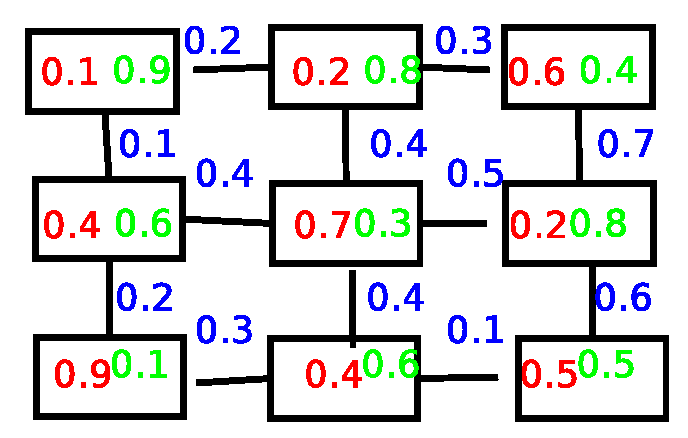
\includegraphics[width=2in]{L10-image-example1.eps}
 \end{figure}
 \begin{itemize}
 \item 
  Red: the probability $f_i$ for pixel $i$ to be foreground; 
  \item 
   Green: the probability $b_i$ for pixel $i$ to be background; 
   \item 
    Blue: the likelihood that pixel $i$ and $j$ are in the same category; 
     \end{itemize}


}

\frame{
\frametitle{ Converting to network-flow problem }
  \begin{figure}
        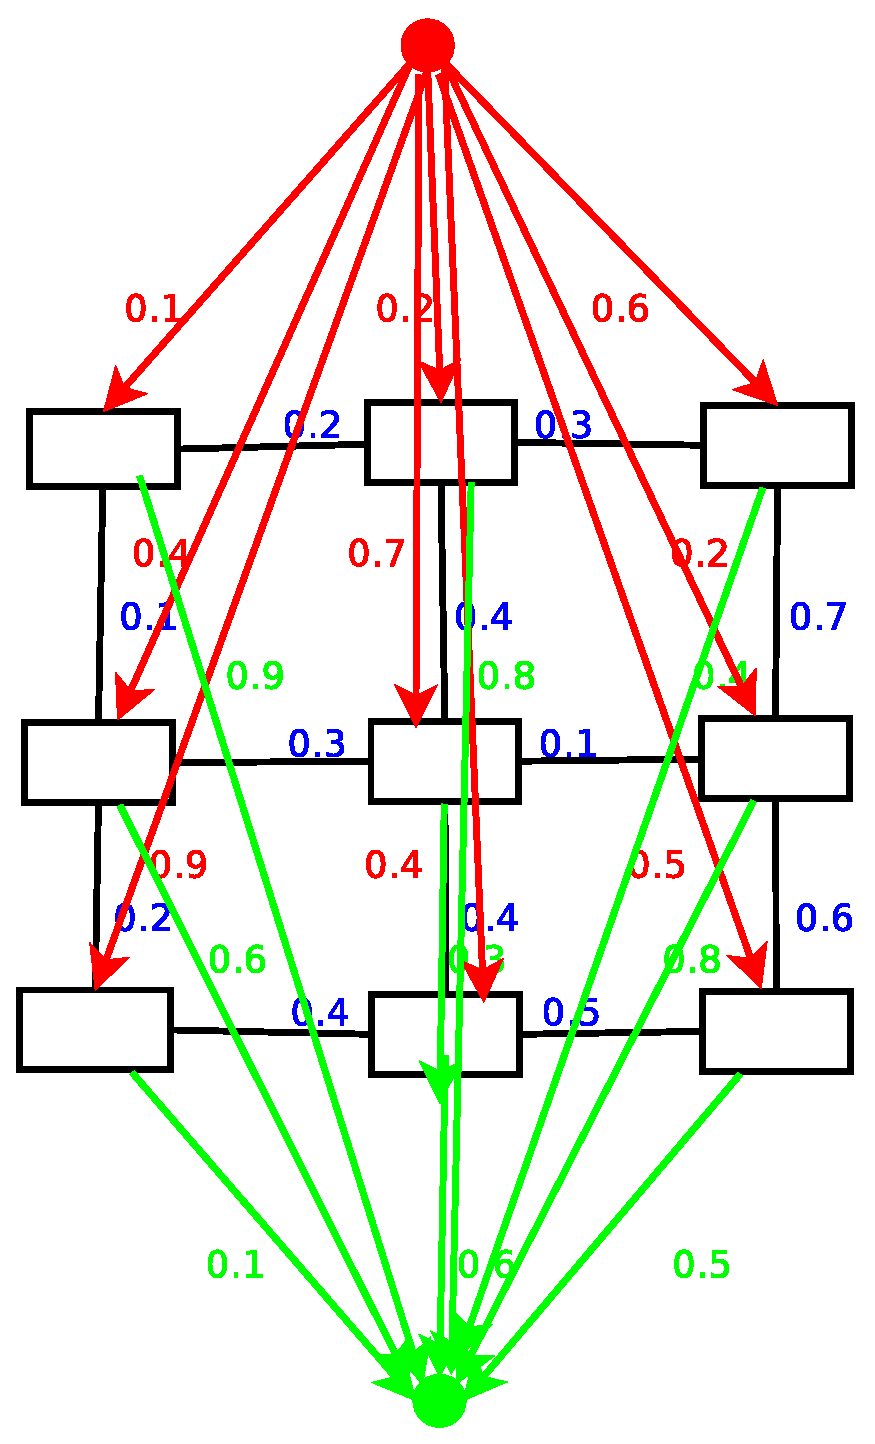
\includegraphics[width=1.2in]{L10-image-example1-network.eps}
  \end{figure}
\begin{scriptsize}
\begin{enumerate}
\begin{small}
 \item Network:  Adding two nodes source $s$ and sink $t$ with connections to all nodes;  
 \item Capacity: $C(s,v)= f_v$, $C(v,t)= b_v$; $C(u,v)=l_{uv}$; 
 \item Cut: a partition.  Cut capacity  $C(F, B) = M - Q(F, B)$, where $M=\sum_i (b_i + f_i) + \sum_i\sum_j l_{ij}$ is a constant.
 \item MinCut: the optimal solution to the original problem
 \end{small}
\end{enumerate}

\end{scriptsize}
}

\frame{
\frametitle{ Problem 2: {\sc Project Selection}  }
\begin{block}{}
{\bf INPUT:} \\ Given a directed acyclic graph (DAG). A node represents a project associated with a profit (denoted as $p_i > 0$) or a cost (denoted as $p_i < 0$), and directed edge $u \rightarrow v$ represent the prerequisite relationship, i.e. $v$ should be finished before $u$. \\
{\bf GOAL: } \\ to choose a subset  $A$ of projects such that: 
 \begin{enumerate}
  \item Feasible: if a project  was selected, all its prerequisites should also be selected; 
    \item Optimal: to maximize profits $\sum_{ v \in A} p_v$; 
 \end{enumerate}
\end{block}

 \begin{figure}
        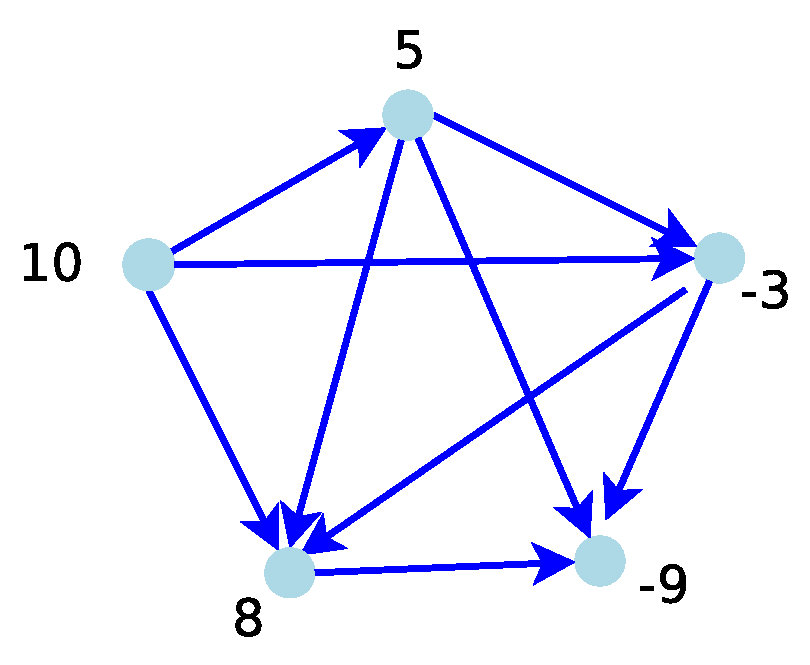
\includegraphics[width=1.3in]{L10-projectselectionexample.eps}
 \end{figure}
}


\frame{
\frametitle{Network construction  }
\begin{figure}
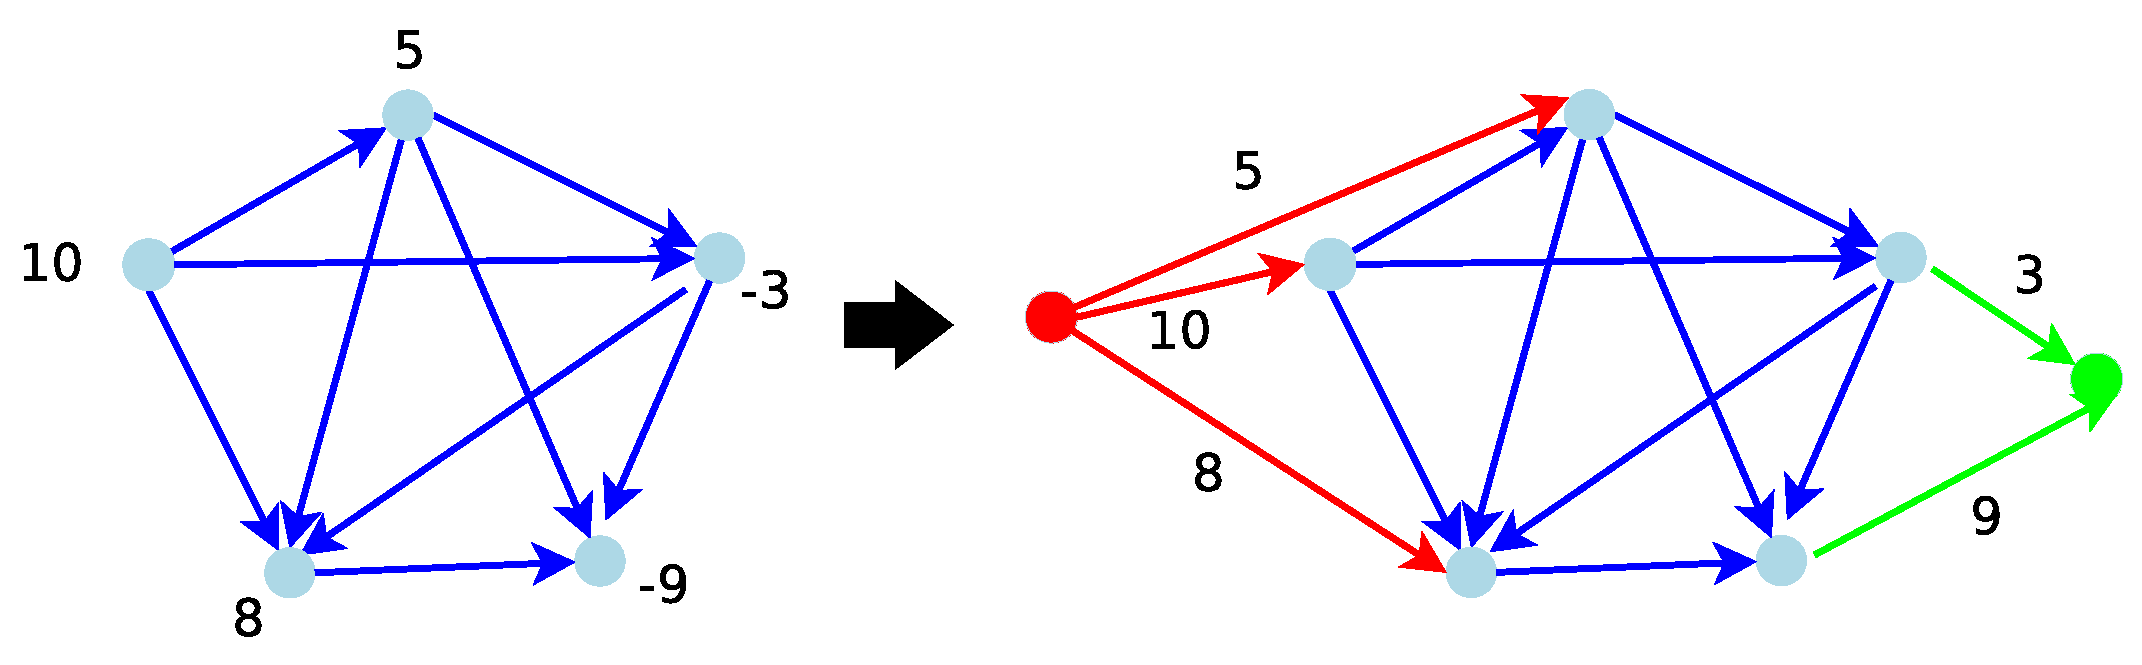
\includegraphics[width=3.3in]{L10-projectselectionexample-network.eps}
\end{figure}


\begin{enumerate}
 \item Network: introducing two nodes: $s$ and $t$, $s$ connecting the nodes with $p_i > 0$, and $t$ connecting the nodes with $p_i < 0$; 
 \item Capacity: moving  weights from nodes to edges, and set $C(u,v)=\infty $ for $<u,v>\in E$. 
 \item Cut: a partition of nodes. 
 \end{enumerate}
}


\frame{
\frametitle{ Minimum cut corresponds to maximum profit }


 
\begin{enumerate}
 \item Cut capacity: $C(A,B) = C - \sum_{i \in A} p_i$, where $C=\sum_{v\in V} p_v $ $(p_v > 0)$ is a constant. 
 \begin{figure}
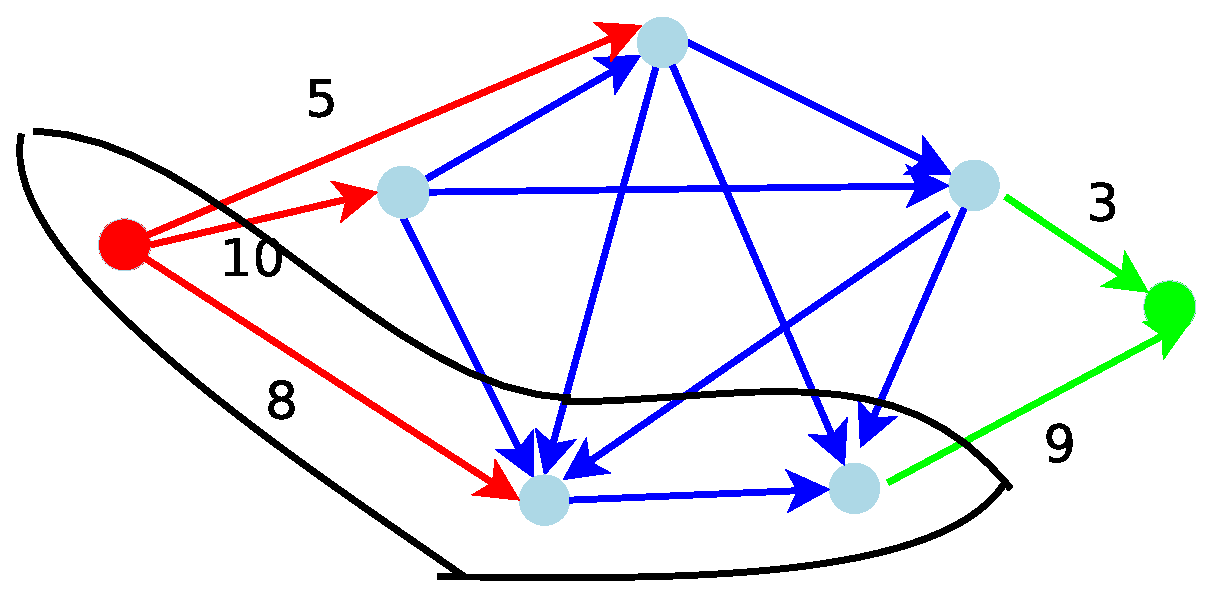
\includegraphics[width=2.5in]{L10-projectselectionexample-network-cut.eps}
\end{figure}
 \item In the example, $C(A,B) = 5 + 10 + 9$, $ \sum_{i \in A} p_i = 8 - 9$, and $C= 5 + 10 + 8$. 
  \item Min-Cut: corresponding to the maximum profit since the sum of cut capacity and profit is a constant. 
\end{enumerate}

} 

\frame{
\frametitle{ Feasibility }
\begin{figure}
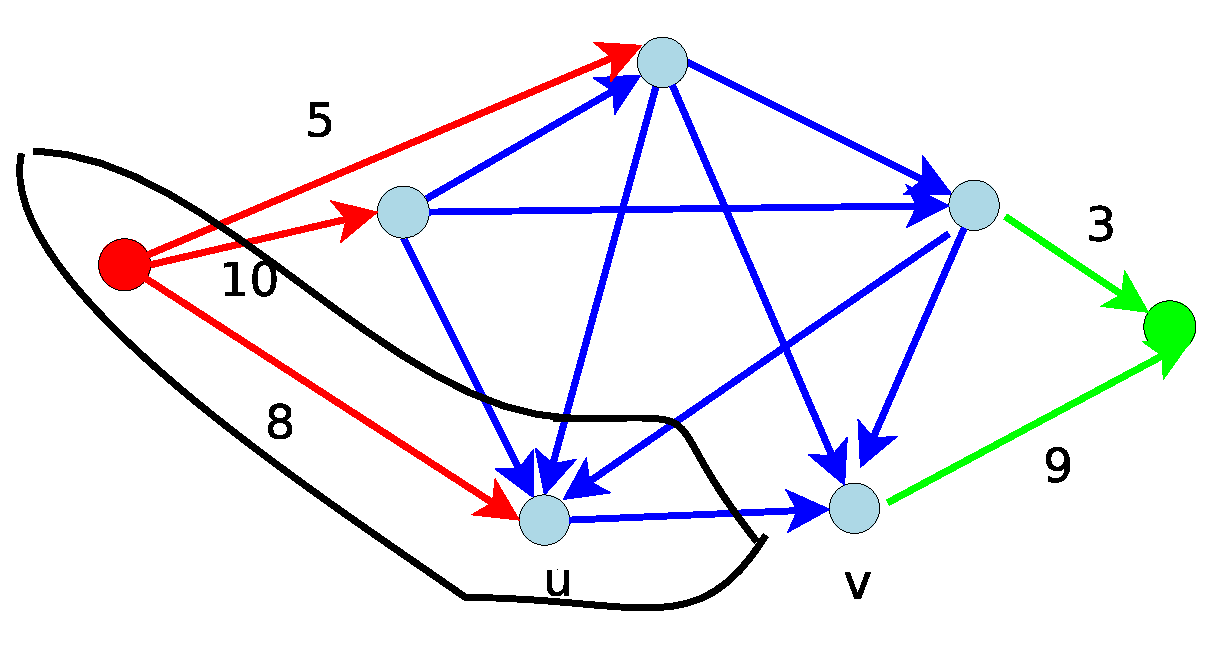
\includegraphics[width=2.5in]{L10-projectselectionexample-network-cut-infeasible.eps}
\end{figure}
\begin{itemize}
\item 
Feasible: The feasibility is implied by the infinite weights on edges, i.e. an invalid selection corresponds to  a cut with infinite capacity. 
\item 
For example, if a project $u$ was selected while its precursor $v$ was not selected, then the edge $<u,v>$ is a cut edge, leading to an infinite cut.
\end{itemize}

} 

\frame{
\begin{block}{}
 Paradigm 2: Finding paths 
\end{block}
}

\frame{
\frametitle{ Problem 3: Disjoint paths } 
\begin{block}{}
{\bf INPUT:} \\ Given a graph $G=<V,E>$, two nodes $s$ and $t$, an integer $k$. \\
{\bf GOAL: } \\ to identify $k$ $s-t$ paths whose edges are disjoint; 
\end{block}
\begin{figure}
        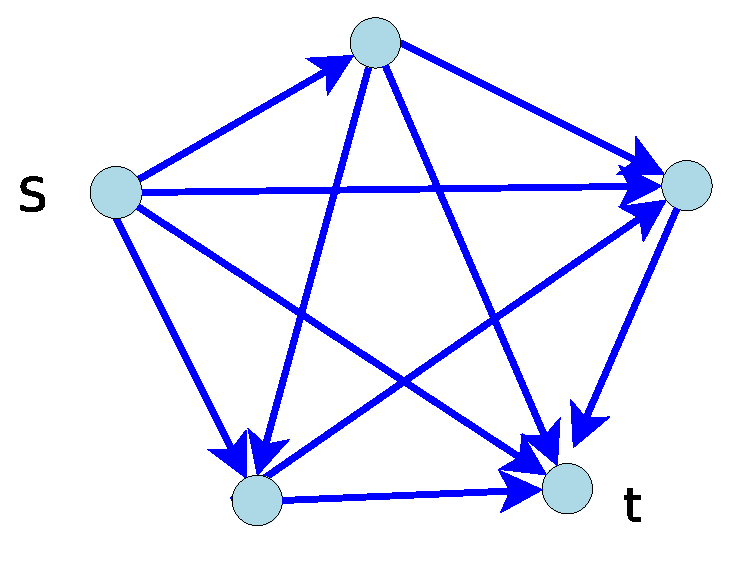
\includegraphics[width=1.5in]{L10-disjointpathsexample.eps}
\end{figure}

Related problem: graph connectivity
}

\frame{
\frametitle{ Network construction   } 
\begin{figure}
        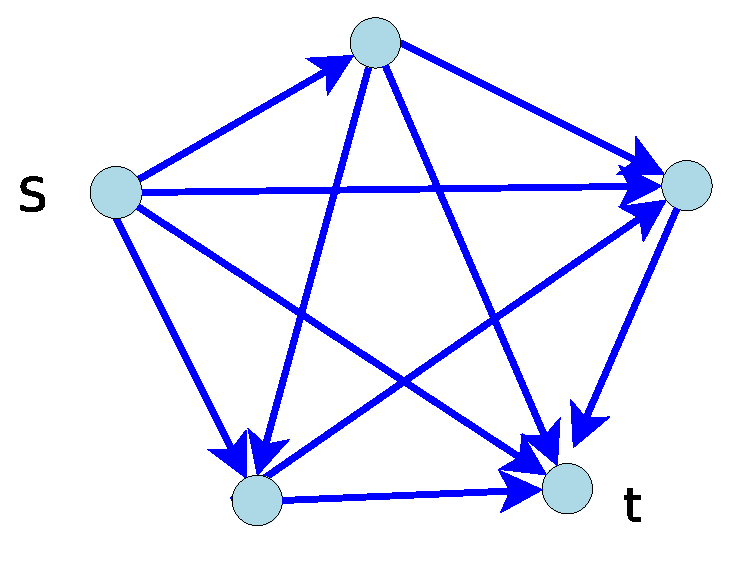
\includegraphics[width=1.3in]{L10-disjointpathsexample.eps}
\end{figure}
\begin{enumerate}
 \item Edges: the same to the original graph;
 \item Capacity: $C(u,v)=1$; 
 \item Flow: (See extra slides)
\end{enumerate}
} 

\frame{


\begin{figure}
        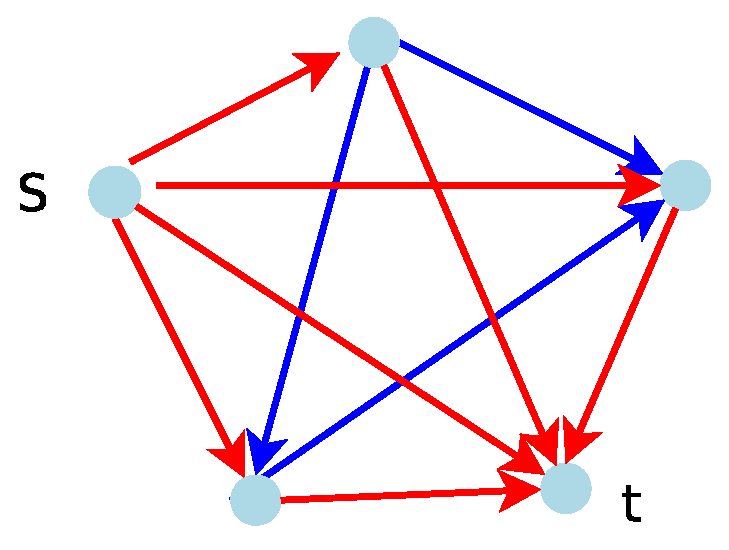
\includegraphics[width=1.3in]{L10-disjointpathsexample-number.eps}
\end{figure}
\begin{Theorem}
$k$ disjoint paths in $G$ $\Leftrightarrow$ the maximum $s-t$ flow value is at least $k$. 
\end{Theorem}
\begin{Proof}
 \begin{enumerate}
  \item Note: maximum $s-t$ flow value is $k$ implies an INTEGRAL flow with value $k$. 
  \item Simply selecting the edges with $f(e) = 1$. 
 \end{enumerate}

\end{Proof}
Time-complexity: $O( mn)$. 
}


\frame{
\frametitle{ Menger theorem 1927  } 

\begin{figure}
        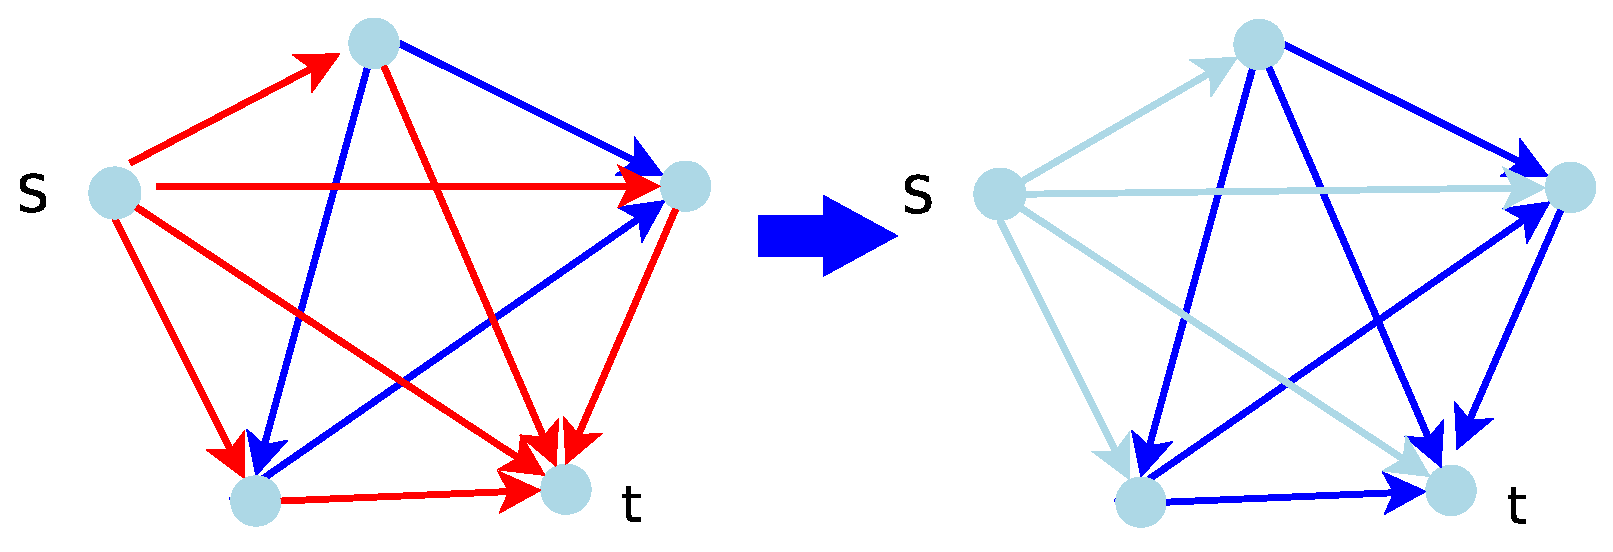
\includegraphics[width=2.7in]{L10-disjointpathsexample-Menger.eps}
\end{figure}
\begin{Theorem}
The number of maximum  disjoint paths is equal to the number of minimal edge removement to separate $s$ from $t$. 
\end{Theorem}
\begin{figure}
        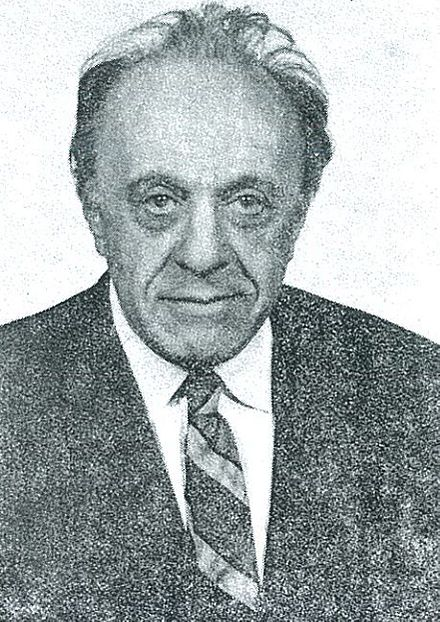
\includegraphics[width=1in]{Menger.jpg}
\end{figure}

}
\frame{
	\frametitle{Menger theorem}
\begin{Proof}
 \begin{enumerate}
  \item The number of maximum  disjoint paths is equal to the maximum flow; 
  \item Then there is a cut $(A,B)$ such that $C(A,B)$ is the number of disjoint paths; 
  \item The cut edges are what we wanted. 
 \end{enumerate}
\end{Proof}
}


\frame{
\frametitle{ Problem 4: Survey design } 
\begin{block}{}
{\bf INPUT:} \\ A set of customers $A$, and a set of products $P$. Let $B(i) \subseteq P$ denote the products that customer $i$ bought. An integer $k$. \\
{\bf GOAL: } \\ to design a survey with $k$ questions such that for customer $i$, the number of questions is at least $c_i$ but at most $c'_i$. On the other hand, for each product, the number of questions is at least $p_i$ but at most $p_i'$. 
\end{block}
\begin{figure}
        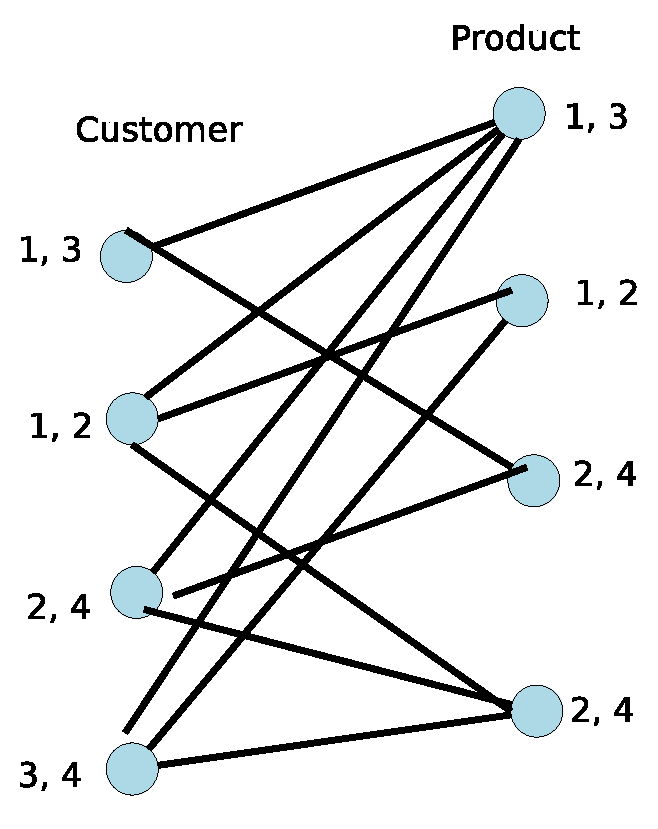
\includegraphics[width=1in]{L10-surveydesignexample.eps}
\end{figure}
}

\frame{
\frametitle{ Network construction } 
\begin{figure}
        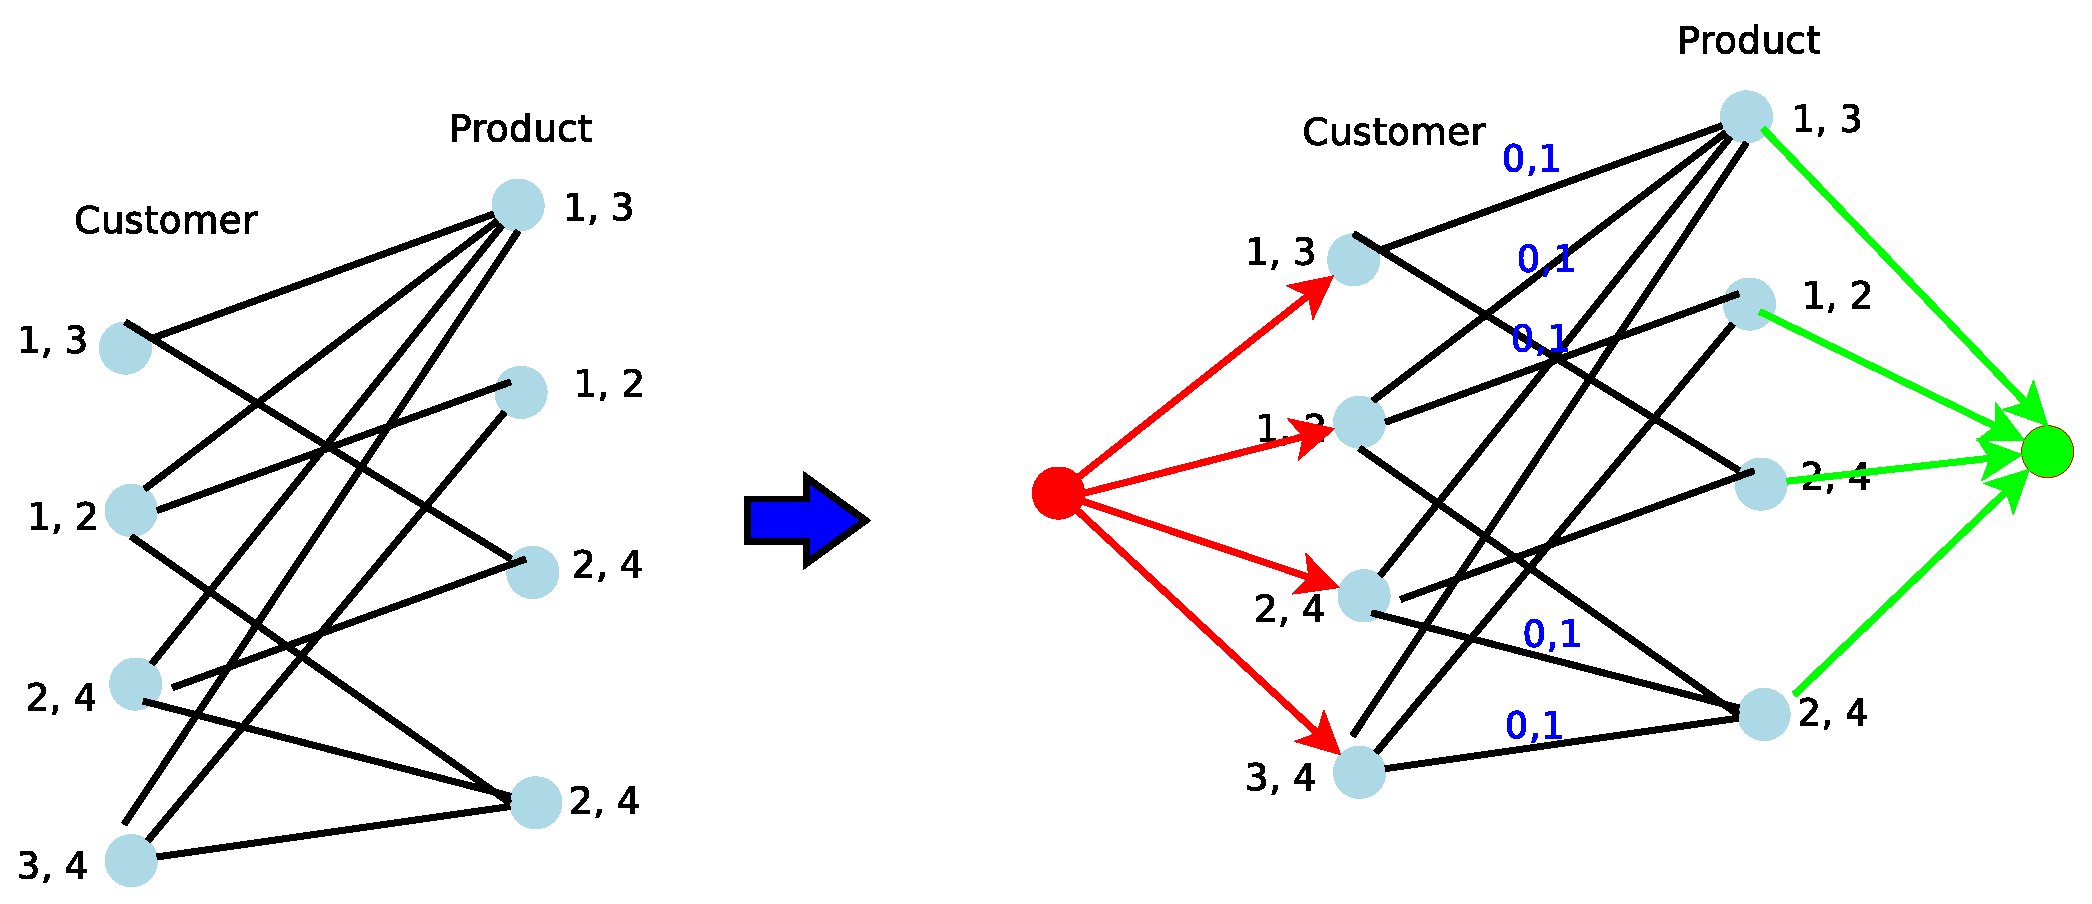
\includegraphics[width=4in]{L10-surveydesignexample-network.eps}
\end{figure}
\begin{enumerate}
 \item Edges: introducing two nodes $s$ and $t$. Connecting customers with $s$ and products with $t$. 
 \item Capacity: moving weights from nodes to edges; setting $C(i,j)=1$; 
 \item Circulation: is a feasible solution to the original problem. 
 \end{enumerate}
}



\frame{
\begin{block}{}
 Paradigm 3: Matching 
\end{block}
}

\frame{
\frametitle{ Problem 5: Matching } 
\begin{block}{}
{\bf INPUT:} \\ A bipartite $G=<V,E>$;\\
{\bf GOAL: } \\ to identify the maximal matching; 
\end{block}
\begin{figure}
        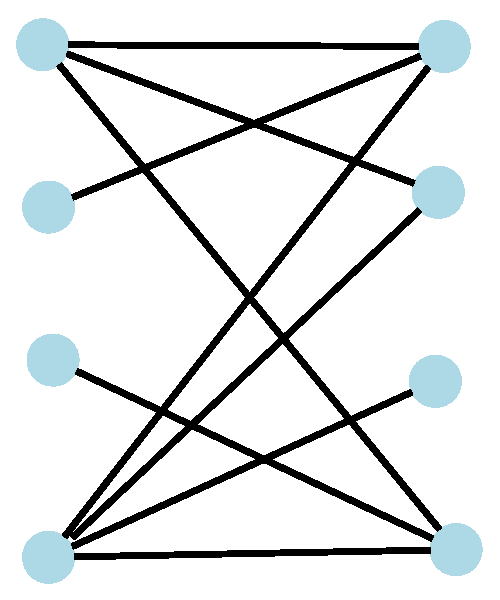
\includegraphics[width=1.in]{L10-matchingexample.eps}
\end{figure}
}


\frame{
\frametitle{ Constructing a network  } 
\begin{figure}
        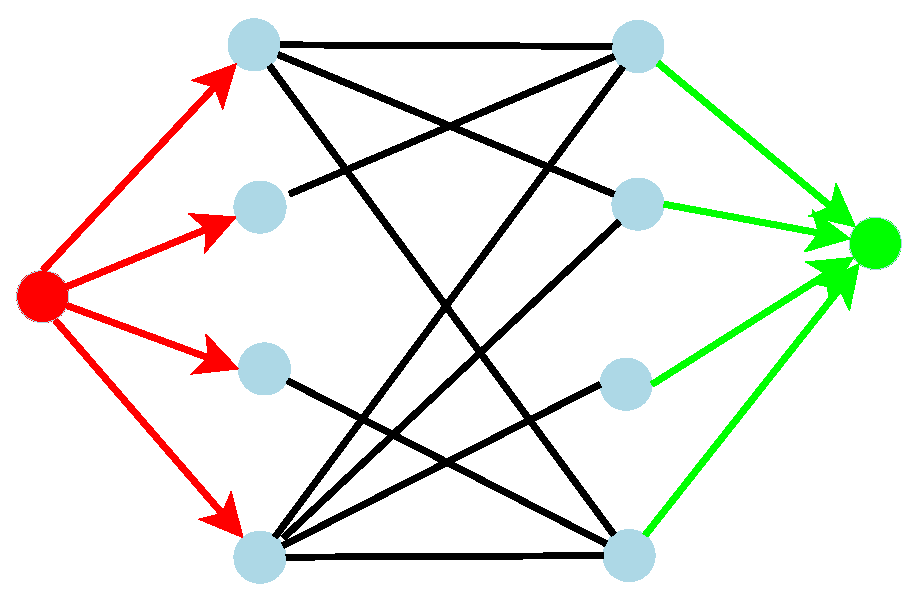
\includegraphics[width=1.5in]{L10-matchingexample-network.eps}
\end{figure}

\begin{enumerate}
\item Edges: adding two nodes $s$ and $t$; connecting $s$ with $U$ and $t$ with $V$; 
\item Capacity: $C(e)=1$ for all $e\in E$; 
\item Flow: the maximal flow corresponds to a maximal matching; 
\end{enumerate}
Time-complexity: $O(mn)$ 
}

\frame{
\frametitle{ Perfect matching:  Hall theorem } 
\begin{figure}
        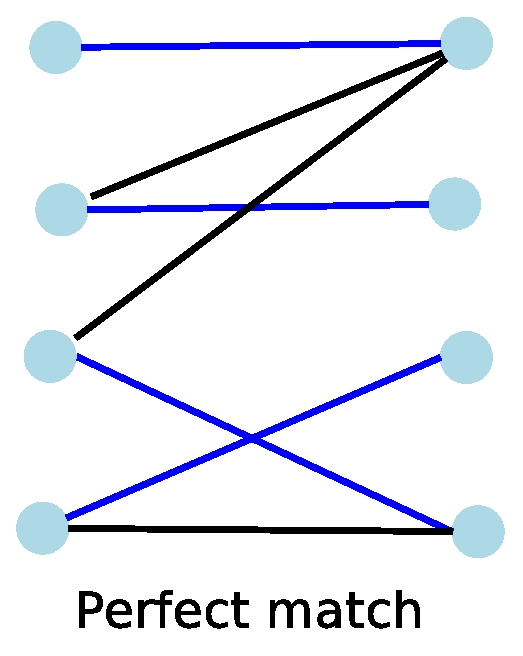
\includegraphics[width=1.in]{L10-perfectmatchingexample.eps}
\end{figure}

\begin{definition}[Perfect match]
Given a bipartite $G=<V,E>$, where $V=X\cup Y$, $X \cap Y = \phi$, $|X|=|Y|=n$. A match $M$ is a perfect match iff $|M|=n$. 
\end{definition} 
} 


\frame{
\frametitle{  Hall theorem, Hall 1935, Konig 1931  } 
\begin{Theorem}
A bipartite has a perfect matching $\Leftrightarrow$ for any $A \subseteq X$, $ |\Gamma(A) | \geq |A|$, where $\Gamma(A)$ denotes the partners of nodes in $A$. 
\end{Theorem}

 \begin{figure}%
   \begin{center}%
     \begin{minipage}{0.30\textwidth}%
      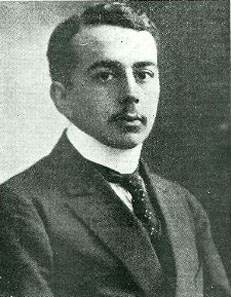
\includegraphics[width=1.0\textwidth]{Konig.jpg}%
     \end{minipage}%
     \quad
     \begin{minipage}{0.30\textwidth}
      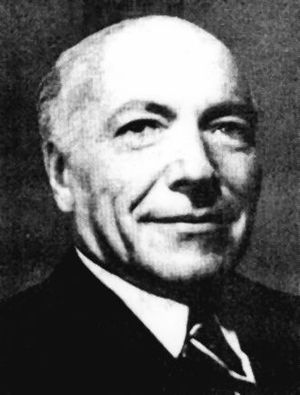
\includegraphics[width=1.0\textwidth]{Egervary.jpg}%
     \end{minipage}%
     \quad
     \begin{minipage}{0.30\textwidth}
      \includegraphics[width=1.0\textwidth]{PhilipHall.jpg}%
     \end{minipage}%     
   \end{center}
   \caption{Konig, Egervary, and Philip Hall}
 \end{figure}

}

\frame{

\begin{figure}
        \includegraphics[width=2.2in]{L10-imperfectmatchingexample.eps}
\end{figure}

\begin{figure}
        \includegraphics[width=1.8in]{L10-imperfectmatchingexampleproof.eps}
\end{figure}
} 

\frame{
\begin{Proof}
Here we only show that if there is no perfect matching, then $ |\Gamma(A) | < |A|$. 
\begin{enumerate}
\item Suppose there is no perfect matching, i.e., the maximal match is $M$, $|M| < n$; 
\item Then there is a cut such that $C(A', B') < n$. Define $A=A'\cap X$;
\item $C(A', B') = | X \cap B' | + | Y \cap A' | = n-|A| + | \Gamma( A ) |$. 
\item We have $ |\Gamma(A) | < |A|$ since $ C(A', B') < n$.   
\end{enumerate}
\end{Proof}

\begin{small} 
Note: If necessary $A'$ can be changed to guarantee that $\Gamma(A)  \subseteq A'$. 

Time-complexity: $O(mn)$ 
\end{small}

}


\frame{
\begin{block}{}
 Paradigm 4: Decomposing numbers 
\end{block}
}

\frame{
\frametitle{ {\sc Baseball Elimination} problem} 
\begin{block}{}
{\bf INPUT:} \\ $n$ teams $T_1, T_2, ..., T_n$. A team $T_i$ has already won $w_i$ games, and for team $T_i$ and $T_j$, there are $g_{ij}$ games left. \\
{\bf GOAL: } \\ Can we determine whether a team, say $T_i$, has already been eliminated from the first place? If yes, can we give an evidence? 
\end{block}

} 

\frame{
\frametitle{ An example } 
 Four teams: \textit{New York, Baltimore, Toronto, Boston} 
\begin{enumerate}
 \item $w_i$: NY (90), Balt (88), Tor (87), Bos (79).
 \item $g_{ij}$: NY:Balt 1, NY:Tor 6, Balt:Tor 1, Balt:Bos 4, Tor:Bos 4, NY:Bos 4. 
\end{enumerate}
It is safe to say that $Boston$ has already been eliminated from the first place since: \begin{enumerate}
\item $Boston$ can finish with at most $79+12=91$ wins.  
\item We can find a subset of teams, e.g. $\{ NY, Tor \}$, with the total number of wins of 90+87+6 = 183, thus at least a team finish with $\frac{183}{2}=91.5 > 91$ wins. \end{enumerate}
Note that $\{NY, Tor, Balt\}$ cannot serve as an evidence that $Bos$ has already been eliminated.

}

\frame{
\frametitle{ {\sc Baseball Elimination} problem } 
\begin{block}{}
Question: For a specific team $z$. Can we determine whether there exists a subset of teams $S \subseteq T-\{z\}$ such that 
\begin{enumerate}
 \item $z$ can finish with at most $m$ wins;
 \item $\frac{1}{|S|} ( \sum\nolimits_{x\in S} w_x + \sum\nolimits_{x,y\in S} g_{xy} )> m $ \nonumber.
\end{enumerate}
In other word, at least one of the teams in $S$ will have more wins than $z$.
\end{block}
}

\frame{
\frametitle{ Network construction: taking $z=Boston$ as an example  } 

\begin{itemize}
 \item We define $m= w_z + \sum_{x\in T} g_{xz} = 91$, i.e. the total number of possible wins for team $z$. 
 \item A network is constructed as follows: 
\begin{enumerate}
 \item Define $S=T-\{z\}$, and $g^*=\sum_{x,y\in S} g_{xy} = 8$.
 \item Nodes:  For each pair of teams, constructing a node ${x:y}$, and for each team $x$, constructing a node $x$. 
 \item Edges:
 	\begin{itemize}
 		\item  For edge $s-{x:y}$, set capacity  as $g_{x,y}$. 
 		\item For edge $x:y-x$ and $x:y-y$, set capacity as $g_{x,y}$. 
 		\item For edge ${x}-t$, set capacity as $m-{w_x}$. 
	\end{itemize}
\end{enumerate}
\end{itemize}
\begin{figure}
        \includegraphics[width=1.9in]{L10-baseballelimination.eps}
\end{figure}
} 

\frame{
\frametitle{ Intuition: number decomposition } 

Intuition: along edge $s-{x:y}$, we send $g_{x,y}$ wins, and at node $x:y$, this number is decomposed into two numbers, i.e. the number of wins of each team. 
\begin{figure}
        \includegraphics[width=1.9in]{L10-baseballelimination.eps}
\end{figure}
} 

\frame{
\frametitle{ Case 1:  the maximum flow value is $g*=8$ } 

\begin{figure}
        \includegraphics[width=1.9in]{L10-baseballelimination.eps}
\end{figure}

\begin{Theorem}
There exist a flow with value $g^*=8$ iff there is still possibility that $z=Boston$ wins the championship. 

\end{Theorem}
}

\frame{
\frametitle{ } 

\begin{figure}
        \includegraphics[width=1.9in]{L10-baseballelimination.eps}
\end{figure}

\begin{Proof}
\begin{itemize}
 \item $\Leftarrow$
 
 \begin{itemize}
 	\item  If there is a flow with value $g^*$, then the capacities on edges $x-t$ guarantees that no team can finish with over $m$ wins.  
	\item Therefore, $z$ still have chance to win the championship (if $z$ wins all remaining games). 
 \end{itemize}
 
  \item $\Leftarrow$ 
  	 \begin{itemize}
 	\item  If there is possibility for $z$ to win the championship 
	\item  we can define a flow with value $g^*$. 
	\end{itemize} 
\end{itemize}
\end{Proof}
} 


\frame{
\frametitle{ Case 2: the maximum flow value is less than $g*=8$ } 

\begin{figure}
        \includegraphics[width=2.in]{L10-baseballeliminationproof.eps}
\end{figure}
\begin{Theorem}
 If the maximum flow value is strictly smaller than $g^*$, the minimum cut describes a subset  $S \subseteq T-\{z\}$ such that 
$\frac{1}{|S|} ( \sum\nolimits_{x\in S} w_x + \sum\nolimits_{x,y\in S} g_{xy} ) > m$ \nonumber.
\end{Theorem}
\begin{Proof}
 (See extra slides)
\end{Proof}
}

 
\frame{
\begin{block}{}
 Extensions of matching: {\sc Assignment} problem, Hungarian algorithm for {\sc Weighted Assignment} problem, Blossom algorithm.
\end{block}
}

\end{document}
